% PBGIA interdisciplinary manuscript -- focused revision, 17 November 2026.
% Journal-neutral article format, NOT a publisher-specific submission template.
% Replace author information and declarations after coauthor approval.
% Preliminary figures. New 2D real-image pilot uses CC0 scikit-image data. The 2D half of Fig. 7 is an analytic illustration.
\documentclass[11pt,a4paper]{article}
\usepackage[margin=1in]{geometry}
\usepackage[T1]{fontenc}
\usepackage[utf8]{inputenc}
\usepackage{lmodern}
\usepackage{amsmath,amssymb,amsfonts,bm,mathtools}
\usepackage{booktabs,tabularx,threeparttable,multirow,array}
\usepackage{graphicx,float,placeins}
\usepackage{caption,subcaption}
\usepackage[numbers,sort&compress]{natbib}
\usepackage{microtype}
\usepackage{siunitx}
\usepackage{xcolor}
\usepackage[colorlinks=true,linkcolor=blue!50!black,citecolor=blue!50!black,urlcolor=blue!50!black]{hyperref}
\usepackage{enumitem}
\captionsetup{font=small,labelfont=bf}
\setlength{\parskip}{0.25em}
\setlength{\parindent}{1.2em}
\newcommand{\nn}{\bm n}
\newcommand{\vv}{\bm v}
\newcommand{\xx}{\bm x}
\newcommand{\dd}{\mathrm{d}}
\newcommand{\bbZ}{\mathbb Z}
\newcommand{\RP}{\mathbb{RP}}
\newcommand{\Sn}{\mathbb S}
\newcommand{\gt}{\mathrm{GT}}
\newcommand{\rel}{\mathrm{rel}}
\newcommand{\energy}{\mathcal E}
\newcommand{\Ham}{\mathcal H}
\newcommand{\degree}{\operatorname{deg}}
\newcommand{\Tr}{\operatorname{tr}}
\newcommand{\MARE}{\mathrm{MARE}}
\newcommand{\diff}{\partial}
\newcommand{\figurepath}[1]{figures/#1.pdf}
\newcommand{\journote}[1]{\textcolor{red!65!black}{[EDITORIAL NOTE: #1]}}

\title{Geometry and projective orientation from binary-field-driven spin textures: A physics-based framework for multidimensional image analysis}
\author{Author list and affiliations to be confirmed by the research team}
\date{Focused interdisciplinary draft --- 17 November 2026}

\begin{document}
\maketitle

\begin{abstract}
Binary images encode boundaries and shapes that can be represented through the collective behavior of a continuous field. Here we develop a physics-based framework in which a binary $\mathbb Z_2$ input acts as a spatial external field and generates a normalized spin texture. A continuum exchange--field model motivates the formation of finite-width domain walls and the proportionality between integrated interfacial energy and boundary extent. On discrete two- and three-dimensional grids, a fixed-iteration spin-field algorithm provides a shared representation for geometric and directional observables. In independent synthetic tests, the selected readouts achieve mean absolute relative errors of $0.893\%$ in perimeter and $0.732\%$ in surface area, while the field also encodes local normals, orientation tensors, and topological degree. Coarse-graining transverse-spin outer products produces a projective director wherever the leading tensor eigendirection is distinguishable. A new stadium study with analytic perimeter and orientation reference yields a mean axial error of $0.21^\circ$ and a $0.93\%$ held-out perimeter error after one reference calibration. We further extend the construction to grayscale images by generating a set of binary fields at multiple intensity thresholds and pooling their orientation tensors. The resulting director maps visualize both local orientation and anisotropy strength in layered and fiber-like patterns; a controlled rotation of a CC0 architectural texture illustrates global orientation tracking. Direct lattice integrations in 2D and compactified preimage counts in 3D provide topology-related checks, while a synthetic 3D fiber array demonstrates orientation extraction from a volume. These results demonstrate a unified spin-texture representation for geometric, directional, and selected topological measurements, complementary to established image-analysis tools.
\end{abstract}

\noindent\textbf{Keywords:} binary images; domain walls; spin textures; geometry estimation; surface area; director fields; projective spaces; topological degree; voxel data.

\section*{Introduction}
The geometry of an object can be described by different quantities: its boundary extent, local surface normal, predominant orientation, connectivity, and topological invariants. Conventional image analysis typically evaluates these properties using distinct operations, such as contour extraction, finite differences, structure tensors, connected-component analysis, and triangulation \cite{Bigun1991,Haralick1979}. Such specialized methods are often efficient and accurate, but they do not necessarily yield a common intermediate representation that can be reused for several tasks. A complementary strategy is to associate an image with a smooth, higher-dimensional field and extract several observables from that field.

A binary image naturally defines a two-state source field. This resembles the spatially varying field acting on a ferromagnetic order parameter: exchange favors a smooth spin texture, the external bias distinguishes the two domains, and a weak chiral coupling can resolve the remaining ambiguity in the orientation of the transverse spin components. The interface between oppositely biased regions becomes a domain wall, which can encode local boundary geometry. Domain walls, chiral interactions, and spin-based topological quantities provide established magnetic motivation \cite{Dzyaloshinskii1958,Moriya1960,Nagaosa2013}. The analogy is useful even when the generated field is employed as a computational representation rather than as a literal model of a magnetic material. Diffuse-interface descriptions of boundary extent and conventional image structure tensors have substantial prior foundations; our aim is not to claim the perimeter principle or orientation-tensor eigenanalysis as a new mathematical discovery \cite{Modica1987,Bigun1991}.

The present work extends a sequence of related studies by our research team, and their respective contributions must be distinguished. An earlier image-to-spin conversion approach transferred chiral textures to grayscale images and used integrated topological charge for image topology and counting applications \cite{Park2024AMT}. Subsequent work generalized the overlay of normalized chiral fields to the estimation of Euler characteristics of multidimensional objects \cite{Moon2025SR}. A separate study introduced a magnetic structure tensor based on spin rotations, with applications to defects, magnetic textures, spiral patterns, and fingerprints \cite{Park2025iScience}. The counting principle, the general idea of an overlaid chiral field, and fingerprint-oriented texture analysis are therefore \emph{prior results}, not new claims of the present article. Here we combine geometric boundary extent, local and spatial orientation, and coarse-grained projective directors within one computational spin representation. We evaluate these observables together with established image-analysis estimators and illustrate an extension to grayscale textures using multiple intensity cutoffs. The resulting framework is a method for generating and reusing orientation-rich geometric representations rather than a replacement for every specialized image-analysis estimator.

Two conceptual distinctions are particularly important. First, the one-dimensional domain-wall solution belongs to an idealized variational model; the accelerated grid-based update evaluated below does not exactly minimize the same Hamiltonian. Second, an unoriented director has no intrinsic arrow and cannot by itself represent material transport. Moreover, projection or averaging of normalized spins generally produces a positive-semidefinite tensor, not automatically a point in real projective space. Maintaining these distinctions makes it possible to evaluate the representation without interpreting numerical convenience as a new physical law.

Our article has two main parts. Section~\ref{sec:theory} outlines the continuum mechanism that connects a binary step field to boundary-localized spin textures and introduces the associated observables. Section~\ref{sec:implementation} reports a specific pixel/voxel implementation and its measured performance. Section~\ref{sec:discussion} discusses the relationship to previous spin-based topology studies, uncertainty caused by rasterization, and the role of possible applications.

\section{Theoretical framework: from binary domains to spin and director fields}\label{sec:theory}
\subsection{A binary source coupled to a normalized order parameter}\label{subsec:theory:model}
Let \(\Omega\subset\mathbb R^d\) be a two- or three-dimensional image domain and let a prescribed binary field be
\begin{equation}
 f(\xx)=\begin{cases}+1,&\xx\text{ inside the object},\\-1,&\xx\text{ outside the object} .\end{cases}
 \label{eq:binary}
\end{equation}
We introduce a \((d+1)\)-component unit field
\begin{equation}
\nn(\xx)=\bigl(\vv(\xx),s(\xx)\bigr)\in\Sn^d,\qquad
\vv\in\mathbb R^d,\quad s\in\mathbb R,\quad |\vv|^2+s^2=1.
\label{eq:spin}
\end{equation}
Thus a two-dimensional input is represented by an \(\Sn^2\)-valued field and a three-dimensional input by an \(\Sn^3\)-valued field. The binary source \(f\) remains fixed while the spin field relaxes. The scalar component \(s\) is favored to approach \(f\) away from the boundary; the transverse components become appreciable in the transition region.

For a conceptual continuum benchmark, consider the energy
\begin{align}
E_{\mathrm{var}}[\nn;f]&=\int_{\Omega}\Bigg[\frac{A}{2}\sum_{i=1}^{d}|\diff_i\nn|^2
+h(1-fs) \notag\\[-0.3em]
&\hspace{2.5cm}+D_{\mathrm c}\bigl(s\nabla\cdot\vv-\vv\cdot\nabla s\bigr)\Bigg]\,\dd^d x,
\label{eq:continuumEnergy}
\end{align}
where \(A,h>0\) and \(|D_{\mathrm c}|\) is assumed weak compared with the exchange--field wall scale. The last term is the familiar interfacial (N\'eel-type) Lifshitz invariant in the physical \(d=2\), three-spin-component setting. For \(d>2\), Eq.~\eqref{eq:continuumEnergy} is a \emph{formal chiral extension} to a \((d+1)\)-component order parameter, not a claim that a physical magnet has more than three spin components. The sign of \(D_{\mathrm c}\) chooses a wall chirality. The distinction between such a continuum energy and the implemented alignment dynamics will be retained throughout.

\begin{figure}[t]
\centering\includegraphics[width=0.98\linewidth]{\figurepath{Fig01_conceptual_pipeline}}
\caption{\textbf{Physics-based geometric representation.} An ideal binary source couples to a normalized spin field. A boundary-localized texture then supports estimates of boundary extent, directional statistics, projective directors, and topological descriptors. The circular example is constructed from a signed-distance profile, so the illustrated wall band has a constant width measured along the local normal rather than along fixed Cartesian axes. The panels are conceptual, not a reconstruction from the final grid benchmark. The full spin projector is \(\nn\nn^{\mathsf T}\), whereas the spatial director uses the transverse vector component \(\vv\).}
\label{fig:pipeline}
\end{figure}

\subsection{One-dimensional domain wall in a step-shaped field}\label{subsec:theory:wall}
The essential mechanism can be demonstrated without solving the full two- or three-dimensional problem. Let \(u\) denote the coordinate normal to a flat input interface, with \(f(u)=\operatorname{sgn}u\). A planar wall is parameterized by
\begin{equation}
 \nn(u)=\bigl(c\sin\theta(u),\cos\theta(u)\bigr),\quad
 c=\pm1,\quad \theta(-\infty)=\pi,\quad\theta(+\infty)=0.
 \label{eq:wallansatz}
\end{equation}
The one-dimensional reduction of Eq.~\eqref{eq:continuumEnergy} is
\begin{equation}
E_{\mathrm{1D}}=\int_{-\infty}^{\infty}\left[\frac A2(\theta')^2
+h\bigl(1-f(u)\cos\theta\bigr)+cD_{\mathrm c}\theta'\right]\dd u.
\label{eq:wallE}
\end{equation}
For prescribed end states the chiral term is a total derivative. The Euler--Lagrange equation is therefore
\begin{equation}
 A\theta''=hf(u)\sin\theta.
 \label{eq:EL}
\end{equation}
Writing \(\ell=\sqrt{A/h}\) and \(q=\tan(\pi/8)=\sqrt 2-1\), the symmetric solution is
\begin{equation}
 \theta(u)=\begin{cases}
 \pi-4\tan^{-1}\!\bigl(q\,e^{u/\ell}\bigr),&u\le0,\\
 4\tan^{-1}\!\bigl(q\,e^{-u/\ell}\bigr),&u\ge0.
 \end{cases}
 \label{eq:wallprofile}
\end{equation}
The spin field is continuous even though its imposed source \(f\) is discontinuous. The length \(\ell\) governs its exponential tails and must not be identified with a particular experimentally measured full width without specifying the width convention.

Using the first integral of Eq.~\eqref{eq:EL}, the nonchiral excess energy per unit boundary extent is
\begin{equation}
 \sigma_0=8\left(1-\frac{1}{\sqrt2}\right)\sqrt{Ah},\qquad
 \sigma(c)=\sigma_0-c\pi D_{\mathrm c}.
 \label{eq:walltension}
\end{equation}
Here the orientation convention in Eq.~\eqref{eq:wallansatz} gives \(\int\theta'\dd u=-\pi\); minimizing over \(c\) yields \(\sigma=\sigma_0-\pi|D_{\mathrm c}|\). This statement applies to the wall within the specified weak-DMI continuum model and does not predict the exact energy of the discrete alignment procedure.

\begin{figure}[t]
\centering\includegraphics[width=.97\linewidth]{\figurepath{Fig02_analytic_wall_scaling}}
\caption{\textbf{A finite-width wall emerges from a discontinuous binary source.} The analytic one-dimensional profile in Eqs.~\eqref{eq:wallprofile} and \eqref{eq:walltension} describes the continuum exchange--field benchmark with the \(A|\theta'|^2/2\) convention. The length \(\ell=\sqrt{A/h}\) and wall energy \(\sigma_0=8(1-1/\sqrt 2)\sqrt{Ah}\) apply at zero DMI; weak chirality selection adds \(\mp\pi D_{\mathrm c}\) for the two wall orientations. A locally flat wall contributes approximately \(\sigma\) per unit boundary extent. This is not an analytic solution of the accelerated grid update used in Sec.~\ref{sec:implementation}.}
\label{fig:wall}
\end{figure}

When the typical radius of curvature \(R_{\rm curv}\) and separations between neighboring interfaces are large compared with the wall width, a curved boundary can be approximated by such locally flat profiles. Its excess energy then scales as
\begin{equation}
 E_{\rm wall}\simeq\sigma\,\mathcal A_{d-1}(\partial\Omega_+),\qquad
 R_{\rm curv}\gg\ell,
 \label{eq:areascaling}
\end{equation}
where \(\mathcal A_{d-1}\) is perimeter for \(d=2\) and surface area for \(d=3\). The proportionality is approximate: curvature, boundary interference, and spatial variations in the wall profile contribute corrections. In particular, Eq.~\eqref{eq:areascaling} motivates a geometric readout but does not imply that physical magnetic energy or the exchange-only gradient integral is an unbiased geometric estimator for arbitrary pixelized objects.

\subsection{Domain-wall orientation, chiral selection, and local geometry}\label{subsec:theory:orient}
For a smooth interface with unit normal \(\bm\nu(\xx)\), a natural local ansatz is
\begin{equation}
 \nn(\xx)\simeq\left(c\sin\theta(u)\,\bm\nu(\xx),\cos\theta(u)\right),
 \label{eq:normalansatz}
\end{equation}
where \(u\) is the signed normal coordinate. Exchange favors spatial coherence, while the chiral invariant fixes the sign of the normal-like transverse component within this model. In two spatial dimensions, \(\nn\in\Sn^2\) can therefore be represented by three spin components, whose in-plane part is normal-like along a sufficiently resolved domain wall.

A convenient geometric observable is the derivative Gram tensor
\begin{equation}
 T_{ij}=\int_{\Omega}\sum_{a=1}^{d+1}\diff_i n_a\,\diff_j n_a\,\dd^dx,
 \qquad I_E=\Tr T.
 \label{eq:gram}
\end{equation}
Its trace measures the integrated variation of the field, while its eigenstructure captures anisotropy of boundary-normal variations. This symmetric positive-semidefinite \(d\times d\) tensor should not be confused with the \emph{chiral magnetic structure tensor} \(\chi_{ij}=(\nn\times\diff_i\nn)_j\) introduced for ordinary three-component magnetic textures in our earlier work \cite{Park2025iScience}. The two constructs encode related but distinct properties; the latter explicitly tracks local spin rotation, whereas Eq.~\eqref{eq:gram} is a Gram tensor of spatial derivatives.

A complementary statistic is the intensity-weighted spatial covariance,
\begin{align}
 \bm\mu&=\frac{\int\rho(\xx)\xx\,\dd^dx}{\int\rho(\xx)\,\dd^dx},\\
 C_{ij}&=\frac{\int\rho(\xx)(x_i-\mu_i)(x_j-\mu_j)\,\dd^dx}
 {\int\rho(\xx)\,\dd^dx},
 \label{eq:cov}
\end{align}
where \(\rho\) is a declared boundary-localized weight. Unlike \(T\), \(C\) carries positional information and can recover the separation axis of otherwise isotropic disconnected objects. The principal axes of \(T\) and \(C\) should not be identified without regard to the shape and the target direction.

The primary extent observables examined below are the exchange-like integral \(I_E\) and a scalar total-variation measure,
\begin{equation}
 I_{\rm TV}=\frac12\int_{\Omega}|\nabla s|\,\dd^dx.
 \label{eq:TV}
\end{equation}
For a monotonic isolated wall connecting \(s=-1\) and \(s=+1\), the normal integral of \(|\diff_u s|/2\) is unity, making total variation approximately proportional to boundary extent without explicit dependence on a fixed wall thickness. By contrast, \(I_E\) depends on wall thickness through \(\int(\theta')^2\dd u\). Both acquire biases after sampling, finite differentiation, and curvature-dependent relaxation.


\subsection{Generalization to spatial dimension \texorpdfstring{$d$}{d} and topology}\label{subsec:theory:topology}
The preceding construction extends formally to \(d\)-dimensional binary domains by using \(d\) transverse components and one scalar component. With an adequately resolved boundary, the wall energy or an appropriately calibrated derivative readout can estimate the \((d-1)\)-dimensional boundary measure. The normalized field \(\nn: \Omega\rightarrow\Sn^d\) also allows a degree to be defined when the domain and boundary conditions provide a suitable compactification. In coordinates, its continuum expression is
\begin{equation}
 Q_d=\frac{1}{|\Sn^d|}\int_{\Omega}\det\!\bigl[\nn,\diff_1\nn,\ldots,\diff_d\nn\bigr]\,\dd^dx,
 \label{eq:degreegeneral}
\end{equation}
with \(|\Sn^d|\) the area of the unit \(d\)-sphere, including orientation. For \(d=2\), this becomes the familiar skyrmion number,
\begin{equation}
 Q_2=\frac{1}{4\pi}\int\nn\cdot\bigl(\diff_x\nn\times\diff_y\nn\bigr)\,\dd x\,\dd y,
 \label{eq:skyrmion}
\end{equation}
while for \(d=3\),
\begin{equation}
 Q_3=\frac{1}{2\pi^2}\int\det\!\bigl[\nn,\diff_x\nn,\diff_y\nn,\diff_z\nn\bigr]\,\dd^3x.
 \label{eq:degree3}
\end{equation}
For a family of separated simply connected components with compatible boundary convention and unit charge per component, the topological degree may count components. However, general shapes can contain holes, connected handles, or overlapping walls; neither \(Q_d=N_{\rm objects}\) nor \(Q_d=\chi(\Omega_+)\) follows for arbitrary images. Topology classifies defects only after specifying the target space and boundary conditions \cite{Mermin1979}. The mapping to Euler characteristics and counting was studied previously \cite{Park2024AMT,Moon2025SR}. Our purpose here is to integrate degree with other readouts of the \emph{same} field rather than to introduce object counting as an independent new method.

\subsection{Fiber averaging and conditional projective directors}\label{subsec:theory:projective}
The full spin has a rank-one projector \(P(\xx)=\nn(\xx)\nn(\xx)^{\mathsf T}\). Its pointwise identification \(\nn\sim-\nn\) represents an element of \(\RP^d\), although the imposed source \(f\) fixes a scalar sign convention and does not itself make the original magnetic model invariant under a global spin reversal at fixed \(f\).

To obtain a spatial orientation independent of sign, we use the transverse part \(\vv\) and define \(Q_v=\vv\vv^{\mathsf T}\). Integrating over a fiber of eliminated coordinates \(\bm u\) and coarse-graining over a transverse window produces
\begin{equation}
 \overline Q(\bm X)=\frac{\displaystyle\int W_\ell(\bm X-\bm X',\bm u)\,\omega(s)\,\vv\vv^{\mathsf T}\,\dd\bm X'\dd\bm u}
 {\displaystyle\int W_\ell(\bm X-\bm X',\bm u)\,\omega(s)\,\dd\bm X'\dd\bm u},
 \label{eq:projector}
\end{equation}
where \(W_\ell\ge0\) represents a chosen averaging window and \(\omega(s)=1\) or \(1-s^2\) is a possible weight. The latter emphasizes domain walls. An averaging scale larger than individual fine structures may reveal common orientation, but it may also mix incompatible directions and suppress directional information.

The resulting \(\overline Q\) is in general a mixed positive-semidefinite tensor, not a rank-one element of \(\RP^{d-1}\). Only where \(\Tr\overline Q>0\) and its largest eigenvalue is nondegenerate can a leading eigenline
\begin{equation}
 [\bm d(\bm X)]\in\RP^{d-1},\qquad \bm d\equiv-\bm d,
 \quad\lambda_1(\overline Q)>\lambda_2(\overline Q)
 \label{eq:director}
\end{equation}
be defined. In 2D this is an \(\RP^1\) director, and in 3D it is an \(\RP^2\) director. Restricting a three-dimensional tensor to a two-component in-plane subblock can also yield an \(\RP^1\) director in a projected image. Unlike a vector field, a director does not define signed flow or motion. Its integral lines are therefore orientation trajectories, not transport streamlines.

\begin{table}[t]
\centering\caption{\textbf{Continuous representations and readouts.} Theoretical definitions and interpretation; no universal estimator accuracy is implied.}\label{tab:framework}
\small\begin{tabularx}{\linewidth}{@{}p{.26\linewidth}X@{}}\toprule
Object or observable & Meaning and mathematical definition\\\midrule
Binary source & \(f\in\{\pm1\}\), specified by the input domain\\
Spin field & \(\nn=(\vv,s)\in\Sn^d\), \(|\nn|=1\)\\
Wall excess energy & \(E_{\rm wall}\simeq\sigma\mathcal A_{d-1}\) in the wide-domain regime\\
Derivative Gram tensor & \(T_{ij}=\int \diff_i\nn\cdot\diff_j\nn\,\dd^dx\)\\
Boundary extent & Calibrated \(\Tr T\), TV or generated level set\\
Projective director & Leading eigenline of averaged \(\vv\vv^{\mathsf T}\) when \(\lambda_1>\lambda_2\)\\
Topological degree & \(Q_d\) of a compactified \(\Sn^d\)-valued field\\\bottomrule
\end{tabularx}\end{table}

\begin{table}[t]
\centering\caption{\textbf{The step-field domain-wall benchmark.} The coefficient \(A\) multiplies \((\theta')^2/2\); alternate exchange-energy conventions change the numerical definition of \(A\).}\label{tab:wall}
\small\begin{tabularx}{\linewidth}{@{}p{.34\linewidth}X@{}}\toprule
Quantity & Continuum step-field result\\\midrule
External field & \(f(u)=\operatorname{sgn}u\)\\
Euler--Lagrange equation & \(A\theta''=hf\sin\theta\)\\
Decay length & \(\ell=\sqrt{A/h}\)\\
Center of wall & \(\theta(0)=\pi/2\)\\
Zero-DMI wall tension & \(8(1-1/\sqrt2)\sqrt{Ah}\)\\
Chirality-selected tension & \(\sigma_0-\pi|D_{\mathrm c}|\)\\
Extent relation & \(E_{\rm wall}\simeq\sigma\mathcal A_{d-1}\), resolved smooth boundaries\\\bottomrule
\end{tabularx}\end{table}

\FloatBarrier
\section{Discrete implementation and geometric applications}\label{sec:implementation}
\subsection{Grid Hamiltonian and the accelerated spin-field update}\label{subsec:impl:algorithm}
For a regular pixel or voxel lattice, an explicit variational discretization can be written as
\begin{equation}
\begin{split}
 \Ham_{\rm lat}=&-J\sum_{\langle i,j\rangle}\nn_i\cdot\nn_j-h\sum_i f_i s_i\\
 &-D_{\rm a}\sum_i \vv_i\cdot Gs_i,
\end{split}
\label{eq:Hgrid}
\end{equation}
where \(G\) is a centered discrete gradient and \(D_{\rm a}\) includes the chosen discretization and sign convention. On a periodic lattice \(G^*=-G\); a true constrained minimization of \(\Ham_{\rm lat}\) therefore couples \(\vv\) and \(s\) reciprocally. In contrast, the chosen fast image-processing dynamics uses the synchronous normalized effective field
\begin{align}
 \bm H_{v,i}^{(t)}&=J\sum_{j\in\mathrm{NN}(i)}\vv_j^{(t)}+D_{\rm a}G[s^{(t)}]_i,
 \label{eq:updatev}\\
 H_{s,i}^{(t)}&=J\sum_{j\in\mathrm{NN}(i)}s_j^{(t)}+h f_i,
 \label{eq:updates}\\
 \nn_i^{(t+1)}&=\begin{cases}\bm H_i^{(t)}/|\bm H_i^{(t)}|,&|\bm H_i^{(t)}|>\varepsilon,\\\nn_i^{(t)},&\text{otherwise.}\end{cases}
 \label{eq:updaten}
\end{align}
Its scalar field omits the reciprocal \(-D_{\rm a}\nabla_G\cdot\vv\) term, and synchronous full alignment does not guarantee a monotonically decreasing \(\Ham_{\rm lat}\). The positive nearest-neighbor sum must not be silently replaced by a Laplacian. Thus Eqs.~\eqref{eq:updatev}--\eqref{eq:updaten} describe a \emph{magnetic-inspired computational relaxation}, not a strict ground-state solver. A separate, projected-gradient comparison of a reciprocal Hamiltonian is used only as a diagnostic.

The input \(f_i\in\{\pm1\}\) is held fixed. The starting spin is built from the Euclidean distance transform of the \emph{rasterized} mask, not from an analytic ground-truth signed distance. In the final evaluated configuration, \(J=D_{\rm a}=1\), \(h=2\), and the synchronous update is applied for \(N=30\) iterations. The generated field uses a centered scalar gradient. A separately optimized, frozen measurement kernel is applied only after generation; it is not the kernel used in the evolution equation. Periodic boundaries are padded so the evaluated objects remain away from domain edges. Additional implementation details appear in Sec.~\ref{sec:methods}.

Figure~\ref{fig:actualtexture} presents an additional direct test on a rotated \emph{stadium}, in which two semicircular caps of radius $R$ are joined by straight segments with cap-center separation $L$. Its exact continuum perimeter is
\begin{equation}
 P_{\rm stadium}=2\pi R+2L,\qquad L=2R\text{ for the illustrated family}.
 \label{eq:stadiumP}
\end{equation}
This geometry supplies independent references for both perimeter and principal-axis angle. All fields are generated with the same $N=30$ normalized alignment dynamics; the new stadium study is separate from the frozen test summarized below. Twelve rotation conditions from $0^\circ$ to $165^\circ$ in $15^\circ$ increments give a mean absolute axial error of $0.214^\circ$ using wall-weighted spatial covariance. A scalar TV calibration fixed from only the $R=9$, $\theta=0^\circ$ reference was carried unchanged to radii $R=11$--25 at three poses per size. Across these 24 held-out cases, the perimeter MARE was $0.931\%$. The measured-vs-true least-squares slope was $1.0087$ with intercept $0.105$ pixels. The fit quantifies scaling and is not itself the calibration rule.

\begin{figure}[t]
\centering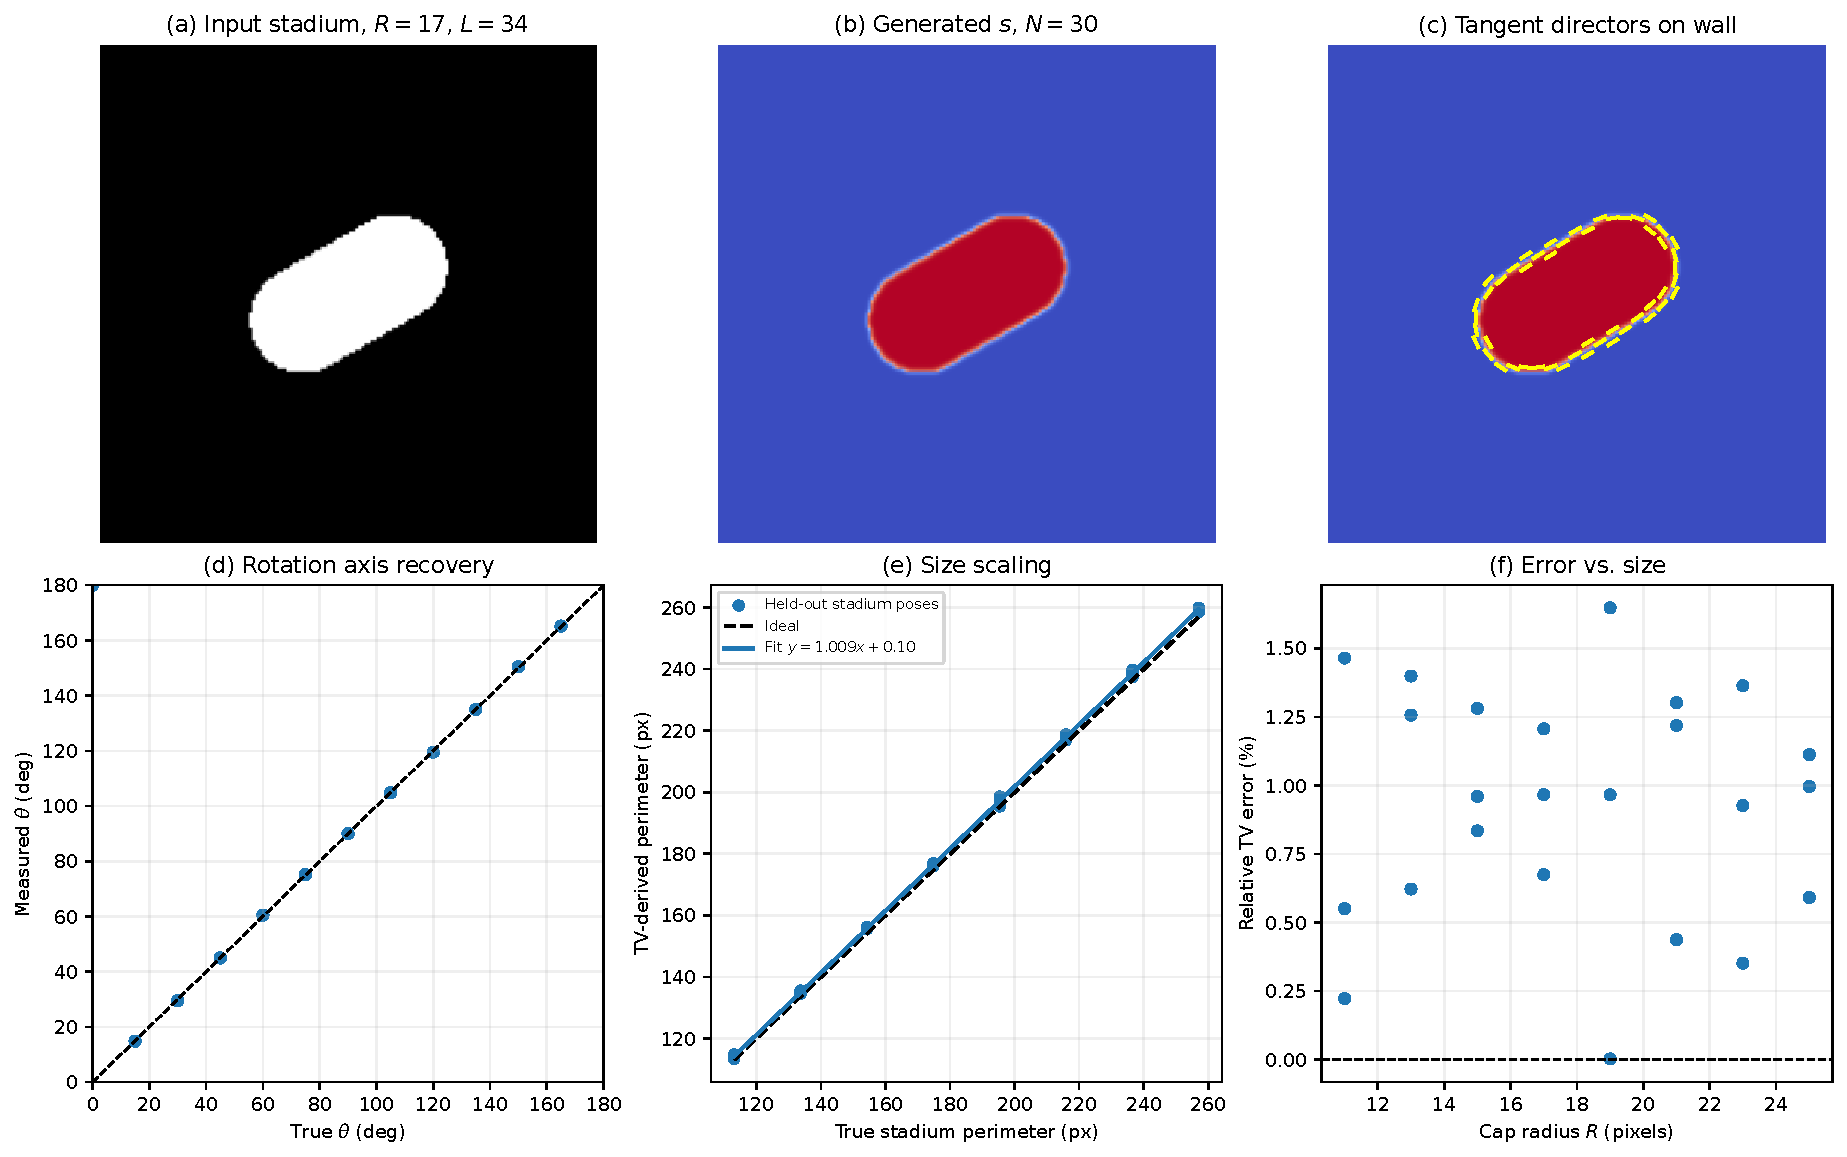
\includegraphics[width=.99\linewidth]{figures/Fig03_stadium_quantitative.pdf}
\caption{\textbf{Analytic stadium geometry validates axis recovery and perimeter scaling from generated spin fields.} (a--c) A rotated binary stadium with $R=17$, $L=34$; its generated scalar field after 30 updates and a wall-localized tangent director. (d) Measured against imposed stadium angle ($0^\circ$--$165^\circ$), with the identity line. (e) TV-derived perimeter against $P_{\rm stadium}=2\pi R+2L$, with the held-out linear fit and identity line. (f) Relative perimeter errors across the held-out sizes; three rotations were tested per radius. The single reference at $R=9$, $\theta=0^\circ$ set the TV conversion coefficient independently of the plotted held-out radii.}
\label{fig:actualtexture}
\end{figure}

The distinction between the algorithm and physical energy is directly testable. In elementary smooth objects the computed Hamiltonian typically decreased during the reported trajectories, but an analytically constructed checkerboard spin configuration increased its energy after one synchronized step by approximately \(1.94\) per site in 2D and \(2.31\) per site in 3D under the reported convention. A reciprocal variational comparison gave monotonically decreasing energy in a restricted demonstration but did not yield better geometric readouts. These observations support interpreting the accelerated dynamics as a representation generator, rather than identifying low magnetic energy with low geometric error.

\subsection{Data design, calibration, and accuracy measures}\label{subsec:impl:benchmark}
The numerical evidence is taken from a frozen final computational study at repository commit \texttt{b2107084d19fcdf54c9350cf3f0e013fed8afa4c}. The independent synthetic benchmark comprises six shape prototypes per spatial dimension in each of training, validation, and test partitions. The 2D families include circles, ellipses, stadiums, rings, nearly touching components, and separated pairs. The 3D families include spheres, ellipsoids, capsules, tori, nearly touching components, and separated pairs. Within each prototype, rotations, subpixel shifts, and noise variants remain in the same partition. The final test contains 72 inputs per dimension, including 24 clean inputs, evaluated on \(80^2\) and \(64^3\) grids, respectively. New shape parameters were used, although not every family was held out entirely from training.

The readout calibration is determined exclusively from separate training-reference circles or spheres. If \(I\) denotes an uncalibrated observable and \(B\) its ground-truth boundary extent, the final estimate is \(\widehat B=cI\), with the fixed scalar coefficient determined by relative least squares across reserved reference shapes. We report mean absolute relative error
\begin{equation}
 \MARE=\frac{100\%}{N_{\rm prototypes}}
 \sum_{p=1}^{N_{\rm prototypes}}\left\langle
 \frac{|\widehat B-B_{\gt}|}{B_{\gt}}
 \right\rangle_{\rm poses\;of\;}p.
 \label{eq:mare}
\end{equation}
Prototype-level aggregation prevents multiple rotations and shifts of the same shape from being treated as independent objects. The final test is not used to set the calibration coefficient or select the readout mixture.

For a bounded final readout comparison, two calibrated observables were combined as
\begin{equation}
 \widehat B_\alpha=\alpha c_E I_E+(1-\alpha)c_{\rm TV}I_{\rm TV},\quad
 \alpha\in\{0,.25,.5,.75,1\}.
 \label{eq:alpha}
\end{equation}
The held-out validation set selected \(\alpha=0\) in 2D and \(\alpha=0.5\) in 3D using a predefined improvement and noise-stability rule. The selection was frozen before the final test. The coefficients and selection rules are released with the code. Here ``selected'' refers to this bounded observer choice, not to a new optimized magnetic Hamiltonian.

\subsection{Perimeter and surface-area estimation}\label{subsec:impl:extent}
Figure~\ref{fig:geometry} and Tables~\ref{tab:extent} and \ref{tab:directiontopology} present the geometric benchmark. The selected readout gave clean-test MARE \(0.893\%\) for 2D perimeter and \(0.732\%\) for 3D surface area. These results show that a shared spin field can support quantitative boundary-extent estimates in both dimensions. Nevertheless, reference-calibrated conventional Crofton and marching-cubes procedures achieved \(0.738\%\) and \(0.563\%\), respectively, on the same clean test (Table~\ref{tab:extent}). Accordingly, the present evidence does not support superiority of the spin approach as a stand-alone perimeter or surface-area estimator.

\begin{figure}[t]
\centering\includegraphics[width=.98\linewidth]{\figurepath{Fig04_geometry_by_family}}
\caption{\textbf{Boundary-extent accuracy varies by shape family and readout.} Prototype-resolved clean mean absolute relative errors from the final independent test. PBGIA readouts use the same \(N=30\) generated field but different frozen observers; conventional comparators use the same train-only calibration policy. The graph shows measured numerical results, not analytically generated values.}
\label{fig:geometry}
\end{figure}


\begin{table}[t]
\centering\caption{\textbf{Boundary-extent estimation on new clean synthetic test prototypes.} MARE values are percent. Unless stated otherwise, readouts use separate train-only calibration with reserved circles/spheres; values are descriptive for the finite test collection.}\label{tab:extent}
\small\begin{tabular}{@{}lrr@{}}\toprule
 Method & 2D perimeter & 3D surface area\\\midrule
PBGIA gradient energy & 1.483 & 0.938\\
PBGIA TV & 0.893 & 0.798\\
PBGIA selected mixture & \textbf{0.893} & \textbf{0.732}\\
Conventional calibrated estimator\tnote{a} & 0.738 & 0.563\\
Generated \(s=0\) contour (raw) & 2.354 & 1.095\\\bottomrule
\end{tabular}
\begin{tablenotes}[flushleft]\footnotesize\item[a] Crofton perimeter in 2D and marching-cubes area in 3D. Raw \(s=0\) has no calibration and is listed separately rather than presented as an equally calibrated method.\end{tablenotes}
\end{table}

Importantly, the modest aggregate benefit from mixing energy and TV did not occur for every shape. For example, in 3D the selected mixture improved the torus error relative to energy alone but worsened the sphere and capsule errors. Paired prototype bootstrap intervals for the improvement included zero in both dimensions, with only six independent test prototypes per dimension. We therefore regard the numerical agreement with conventional geometry estimates, rather than a universal numerical improvement, as the principal result of this benchmark.

The shared field also appears less sensitive to the specific salt-and-pepper corruption used in the benchmark than raw boundary extraction, which counts isolated flipped pixels as additional boundary fragments. Such behavior should not be generalized to arbitrary noise: some denoised conventional methods performed competitively, and alternative filters, thresholds, and noise models were not exhaustively optimized. Computational efficiency also favors direct image methods on the measured CPU: the full PBGIA pipeline required approximately \(13.9\,\mathrm{ms}\) for \(80^2\) inputs and \(584\,\mathrm{ms}\) for \(64^3\) inputs, compared with submillisecond 2D Crofton and a few milliseconds for 3D marching cubes. The PBGIA timings, however, include generation of the common field and multiple readouts.

\subsection{Surface normals and global directions}\label{subsec:impl:directions}
The transverse field is well aligned with smooth input boundaries in the tested resolution regime. On a narrow boundary band, the signed mean cosine of \(\vv\) with the inward analytic normal was \(0.99378\) in 2D and \(0.99667\) in 3D. Errors of selected orientation axes obtained from the derivative Gram tensor were below one degree for elongated ellipse/stadium and ellipsoid/capsule test shapes (Table~\ref{tab:directiontopology}). Spatial covariance gave similarly small errors in these shapes and more directly recovered the center-to-center orientation of disconnected pairs.

This distinction is information-theoretic rather than merely numerical. A pair of widely separated circular objects has a well-defined separation direction in the spatial distribution, while the local normal directions on each circular boundary are nearly isotropic. The local normal tensor cannot be expected to encode their positional separation. Conversely, normal-orientation tensors are appropriate for estimating an orientation distribution when the relevant directional signal is carried by boundary normals rather than by the object's overall spatial extent.

\subsection{Synthetic 3D volume readouts: interface area and fiber axes}\label{subsec:impl:3dvolume}
We extended the fixed-iteration generator to a new set of $68^3$ synthetic volumetric masks with known analytic surfaces. To make the comparison transparent, a single sphere with radius $R=12$ fixed the scale of a central-difference gradient integral; the coefficient was then held fixed for the capsule, torus, pair of spheres, and an array of four separated rounded fibers. These newly generated fields are independent of the frozen shape-family benchmark in Table~\ref{tab:extent}. Relative errors against analytic surface areas were $+1.15\%$ (capsule), $-1.34\%$ (solid torus), $+0.74\%$ (sphere pair), and $-2.45\%$ (fiber array). The corresponding areas and marching-cubes readouts are provided in the reproducibility CSV.

For a long fiber the transverse-spin outer-product tensor is dominated by \emph{surface normals}. Consequently, its \emph{minimum}-eigenvalue axis, rather than its maximum-eigenvalue axis, estimates the fiber longitudinal direction. In the four-fiber array with a prescribed common direction, this readout yielded an axial error of $3.76^\circ$. This volume-level demonstration illustrates the same tensor formalism in three spatial dimensions without assuming that the global largest-eigenvalue direction is the fiber axis. A volume rendering in Supplementary Fig.~\ref{fig:3Dvis} depicts a 3D interface together with the physical three-component transverse vector; the fourth spin component is encoded by the scalar field and its level surface.

\begin{table}[t]
\centering\caption{\textbf{Synthetic 3D geometry and degree from newly generated $S^3$ fields.} Surface-area estimates use a single sphere reference calibration, held fixed for all other shapes; the 3D degree uses a compactified regular-value preimage calculation. The fiber sample consists of four separated rounded fibers, and its orientation readout uses the minimum eigenvector of the transverse normal tensor.}
\label{tab:3dnew}
\small\begin{tabular}{@{}lrrr@{}}\toprule
Volume & Analytic area (voxel$^2$) & PBGIA area error (\%) & $S^3$ degree \\\midrule
Sphere (reference) & 1809.56 & 0.00 & 1\\
Capsule & 1859.82 & +1.15 & 1\\
Solid torus & 2763.49 & $-1.34$ & 0\\
Sphere pair & 2513.27 & +0.74 & 2\\
Four fibers & 3590.97 & $-2.45$ & 4\\\bottomrule
\end{tabular}
\end{table}

\subsection{Coarse-grained projective director fields}\label{subsec:impl:rp}
To probe the proposed \(\Sn^d\rightarrow\RP^{d-1}\) direction representation, six generated 3D textures (sphere, capsule, torus, pair, ellipsoid, and shell) were averaged along three coordinate axes. The study compared the full projector \(\nn\nn^{\mathsf T}\), the amplitude-preserving transverse tensor \(\vv\vv^{\mathsf T}\), uniform averaging, and the wall weight \(1-s^2\). It produced 72 projection tensor maps and an additional 36 in-plane subblock director maps. The averaged tensors were usually mixed: their rank and purity were not equivalent to those of a single projective point.

An instructive negative result arose for the full projector with uniform weights. Its leading eigenline was defined over essentially the full projected maps, but the mean squared scalar component of that eigenvector was \(0.99948\). The apparent high coverage therefore reflected bulk poles with \(s\simeq\pm1\), not useful spatial orientation. The vector or wall-weighted versions reduced this dominance, but valid director coverage depended strongly on projection axis and on the eigenvalue gap. In the torus example, the fraction of valid wall-weighted in-plane directions was approximately \(0.62\), \(0.53\), and \(0.49\) for the three projection axes. Thus the coarse-grained field is a \emph{conditional} director representation rather than a universally defined map.

\subsection{Multithreshold orientation fields and controlled image-level demonstrations}\label{subsec:impl:imagepilot}
Gray-scale or color images generally contain more than one relevant intensity level. Instead of converting an entire image into a single mask, we analyze an image $g(\xx)$ through a \emph{stack} of binary inputs. For a color input we first use a stated luminance conversion; alternative channel-specific analyses are possible but were not tested. After mild Gaussian smoothing, five fixed image-quantile cutoffs ($15$, $32.5$, $50$, $67.5$, and $85$ percent) define $f_k(\xx)=2\mathbf{1}[g(\xx)>t_k]-1$, where $k=1,\ldots,K$ and $K=5$. Independent $N=30$ spin fields $\nn^{(k)}=(\vv^{(k)},s^{(k)})$ are generated using the same parameters and no image-specific trained kernels. The orientation information is pooled at the \emph{tensor} level:
\begin{equation}
 M^{\rm multi}_{ij}(\xx)=\frac{1}{K}\sum_{k=1}^{K}
 \left[G_\sigma*(v^{(k)}_i v^{(k)}_j)\right](\xx),
 \qquad \sigma=8\;\text{pixels}.
 \label{eq:multiimage}
\end{equation}
This positive-semidefinite sum preserves sign invariance of each director candidate and avoids cancellation from adding vectors whose signs differ. The tangent director $[\bm d_\perp]$ is chosen perpendicular to the principal eigenvector of $M^{\rm multi}$; equivalently, it is the eigenline of the smaller eigenvalue of the in-plane normal tensor. We write $\lambda_1\ge\lambda_2\ge0$, $\Delta\lambda=\lambda_1-\lambda_2$, and $c=\Delta\lambda/(\lambda_1+\lambda_2+10^{-12})$. The tensor gap is an anisotropy \emph{strength}, whereas $c$ describes relative directional coherence.

For the plotted directors we sample the field every six pixels, retain positions with $c>0.25$ and a normalized gap of at least $0.07$, and draw undirected segments without arrowheads. The displayed segment length is
\begin{equation}
 \ell_{\rm draw}(\xx)=1.4+9\;\mathrm{clip}\!\left(\frac{\Delta\lambda(\xx)}{\Delta\lambda_{95}},0,1\right)
 \quad\text{pixels},
 \label{eq:segmentlength}
\end{equation}
where $\Delta\lambda_{95}$ is the 95th percentile of the full image's tensor-gap field. The additive $1.4$ pixels improves legibility only for displayed segments; segment \emph{strength} and eligibility are determined by $\Delta\lambda$. This visualization does not rescale the physical spin or the measured tensor. Figure~\ref{fig:directors} displays the intensity input, tensor gap, and dense amplitude-coded directors for three synthetic texture families: curved geological layers, collagen-like fibers, and a leaf-vein analog. They are methodological \emph{illustrations}, not validated tissue, geology, or botany measurements.

The synthetic curved layers offer a known analytical tangent field. On the selected pixels, the multi-threshold PBGIA orientation has a mean absolute axial error of $1.55^\circ$, compared with $0.51^\circ$ for the direct grayscale structure tensor. Beyond this quantitative example, Fig.~\ref{fig:directors} visualizes the spatial variation of direction and tensor anisotropy in representative layered, fibrous, and branching patterns. Further synthetic and CC0 examples appear in Supplementary Fig.~\ref{fig:suppmulti}. A woven texture contains two competing directional families, whereas the leaf-vein analog includes both internal line segments and the outer leaf contour; these cases illustrate how the observable depends on the pattern and its segmentation.

\begin{figure}[t]
\centering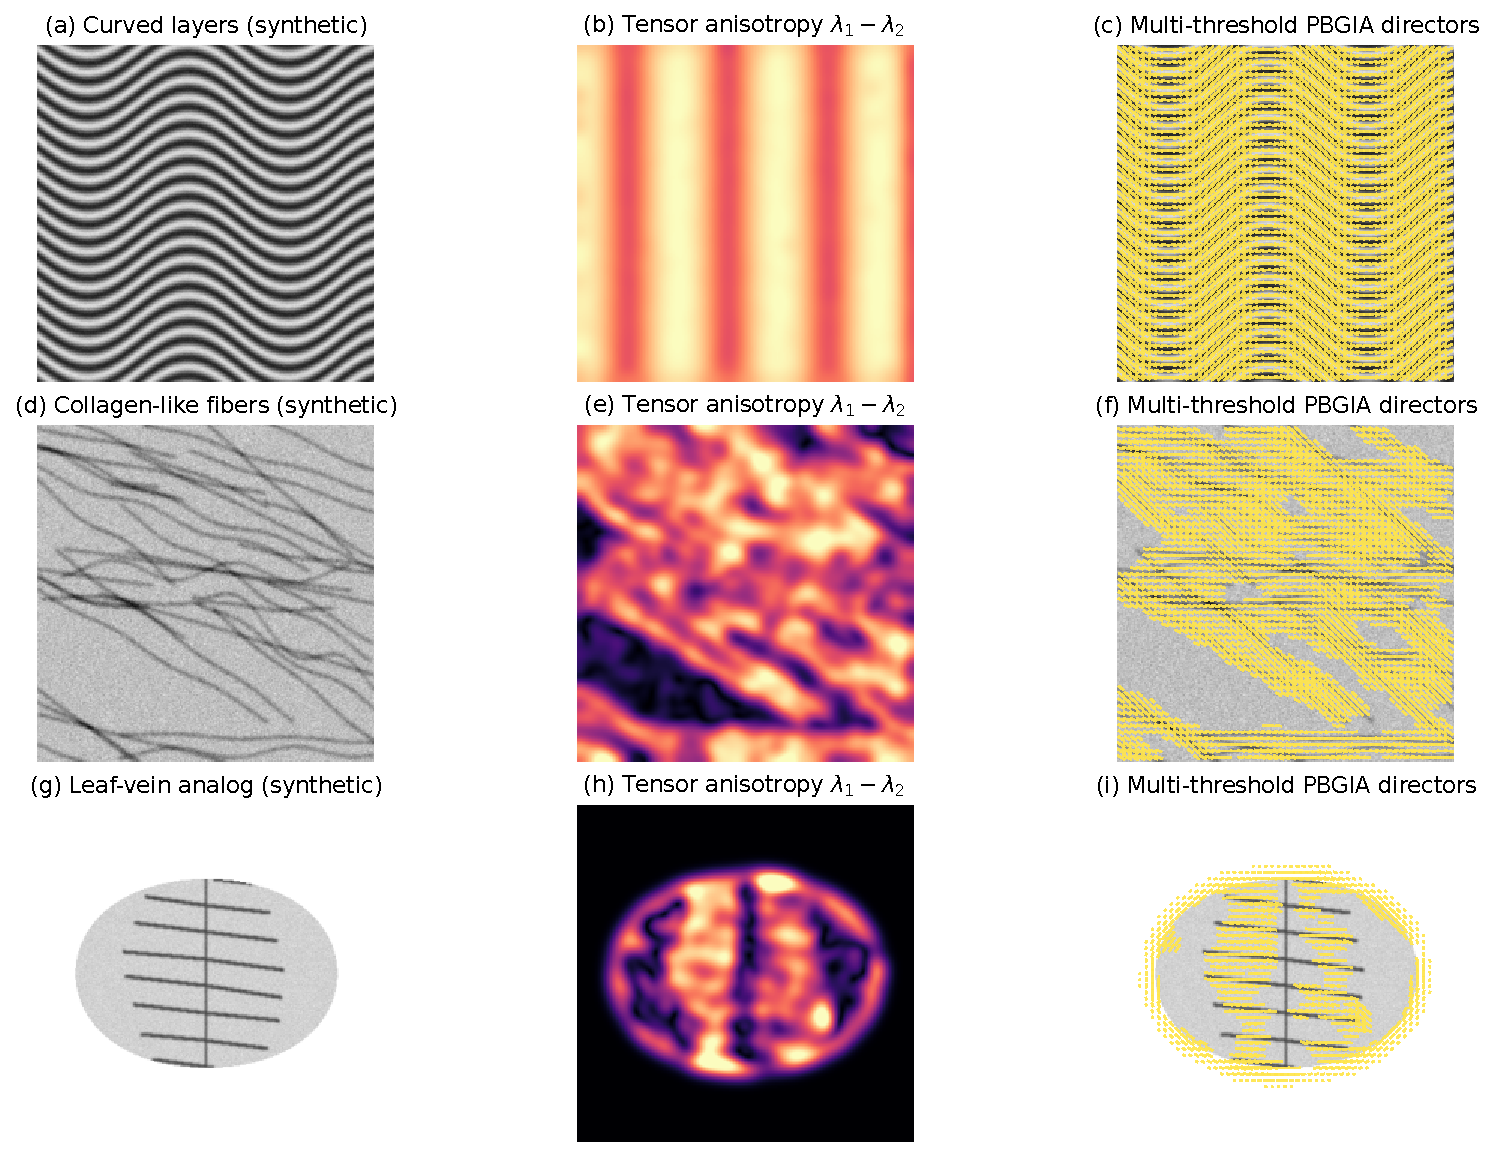
\includegraphics[width=.99\linewidth]{figures/Fig06_multithreshold_directors.pdf}
\caption{\textbf{Multithreshold binary-to-spin conversion yields dense, tensor-strength-scaled director maps.} Each grayscale input is converted into five binary maps at fixed intensity quantiles. For each map, a separate normalized spin texture is generated, and the resulting transverse outer-product tensors are averaged before eigendecomposition. Rows show (a--c) analytically curved synthetic layers, (d--f) synthetic collagen-like fibers, and (g--i) a synthetic leaf-vein analog. Columns show input intensity, the tensor anisotropy $\lambda_1-\lambda_2$, and the tangent director segments. Segment \emph{length} increases with normalized tensor anisotropy; coherence and signal thresholds suppress unreliable directions. All three inputs are controlled synthetic textures; the layered case has an analytic tangent reference, while the collagen- and leaf-like panels visualize candidate director applications.}
\label{fig:directors}
\end{figure}

We also examined the \emph{rotation equivariance} of the global orientation descriptor using the CC0 brick-wall texture from \texttt{skimage.data.brick()}. Known image-plane rotations of $-15^\circ$ to $+15^\circ$ were applied in $5^\circ$ increments, and the resulting change in the estimated axis was compared with the imposed rotation. The mean absolute \emph{relative rotation-tracking error} over seven trials was $2.46^\circ$ for the multi-threshold PBGIA tensor and $0.74^\circ$ for the direct grayscale structure tensor. For the $+10^\circ$ example, the estimated PBGIA axis shift was $+12.83^\circ$ (Fig.~\ref{fig:deskew}). Because the unrotated photograph has no independently labeled physical vertical or unique true axis, this experiment measures rotational consistency, not absolute structural orientation accuracy.

\begin{figure}[t]
\centering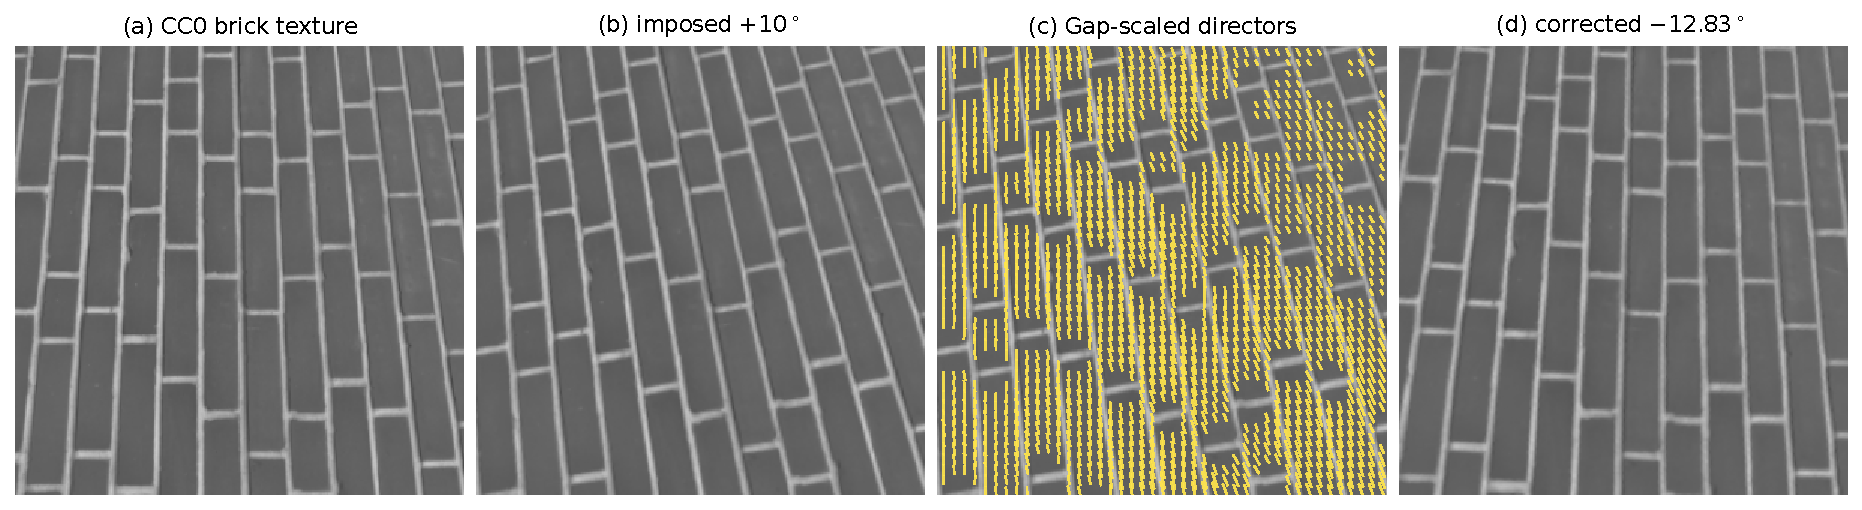
\includegraphics[width=.99\linewidth]{figures/Fig09_multithreshold_deskew.pdf}
\caption{\textbf{Global orientation readout and controlled relative deskew of a CC0 architectural texture.} (a) Original brick texture; (b) image rotated by $+10^\circ$; (c) densely sampled PBGIA tangent directors with lengths proportional to the anisotropy gap of the summed five-threshold tensor; (d) correction by the inferred $-12.83^\circ$, displayed after cropping all panels to the same central $258\times258$ pixel region that excludes rotation-generated border pixels. Across seven imposed rotations, the mean absolute \emph{relative rotation-tracking error} was $2.46^\circ$ for PBGIA and $0.74^\circ$ for a direct grayscale structure tensor. The image has no independently labeled absolute orientation. Source: \texttt{skimage.data.brick()} (CC0Textures/Bricks25 material, CC0); cropping, rotation, and overlays are our modifications.}
\label{fig:deskew}
\end{figure}

\subsection{Topological descriptors from numerically generated fields}\label{subsec:impl:topology}
The same 30-step algorithm was applied to four newly constructed 2D binary masks: one disk, two disks, an annulus, and a separated disk--annulus pair. Rather than plotting analytic skyrmion configurations, we integrated the \emph{actual generated} $S^2$ fields using the oriented solid angles of the two spherical triangles associated with each square plaquette. The resulting $Q_2$ values were $1.0000000$, $2.0000000$, $0.0000000$, and $1.0000000$, respectively (Fig.~\ref{fig:topology}). In these tested shapes $Q_2$ equals the binary Euler characteristic $\chi$, while it counts connected components only in the no-hole cases. The topological counting principle was established in earlier papers by this group \cite{Park2024AMT,Moon2025SR}; here the value of the calculation is its joint availability with geometry and director readouts.

\begin{figure}[t]
\centering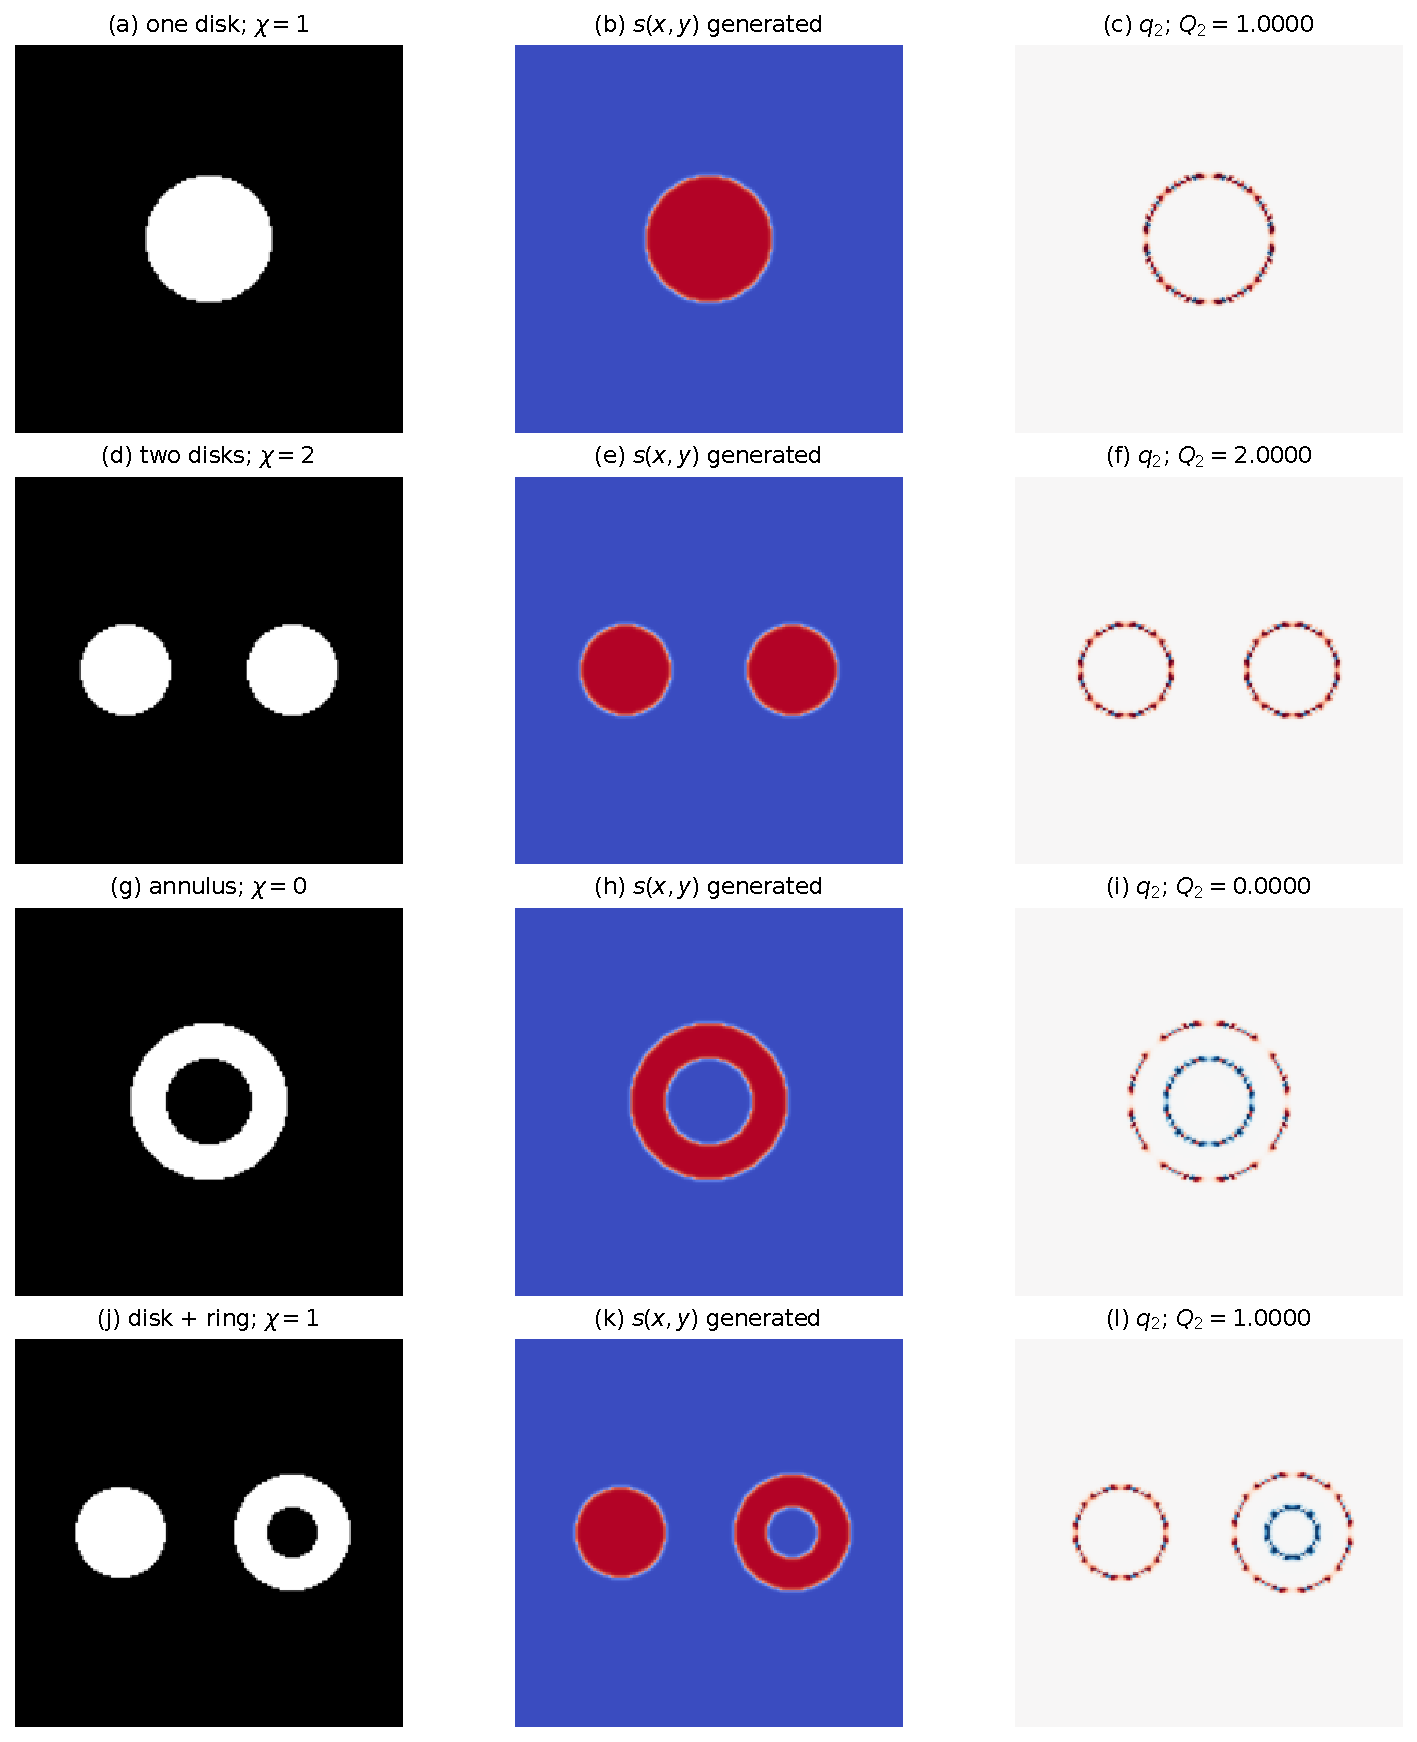
\includegraphics[width=.93\linewidth]{figures/Fig07_2D_generated_Q2.pdf}
\caption{\textbf{Two-dimensional topological readout computed from actual 30-step spin fields.} For each row, the binary mask, generated $s$ component, and finite-difference topological density are shown for (a--c) one disk, (d--f) two disks, (g--i) an annulus, and (j--l) a disk--annulus pair. The charge $Q_2$ printed in the right panel was evaluated from a separate oriented spherical-triangle quadrature over the generated $S^2$ spin field; it was not assigned analytically or computed by direct connected-component labeling. The corresponding raster Euler characteristics are $1,2,0,1$.}
\label{fig:topology}
\end{figure}

In three dimensions, the generated $S^3$ field is compactified by a constant outer collar, a cubic cell is divided into six oriented tetrahedra, and the normalized piecewise-linear interpolation is tested against a generic regular target value. The signed regular-value preimage count yields degrees $1,1,0,2$ for sphere, capsule, solid torus, and separated sphere pair in the newly generated $68^3$ examples (Fig.~\ref{fig:3Dtopo}); a four-fiber array yielded degree $4$ (Table~\ref{tab:3dnew}). Repeating the regular-value calculation with three distinct generic target vectors gave identical degrees for all five analytically defined volume families. These match the corresponding simple synthetic-volume Euler characteristics under the tested conventions, consistent with the earlier numerical topological method \cite{Moon2025SR}. This discrete preimage method should be distinguished from a coarse-grid finite-difference determinant integral, which has substantial quadrature bias at the present wall resolution. Figure~\ref{fig:3Dtopo} shows both outputs instead of implying that the latter is already converged.

\begin{figure}[t]
\centering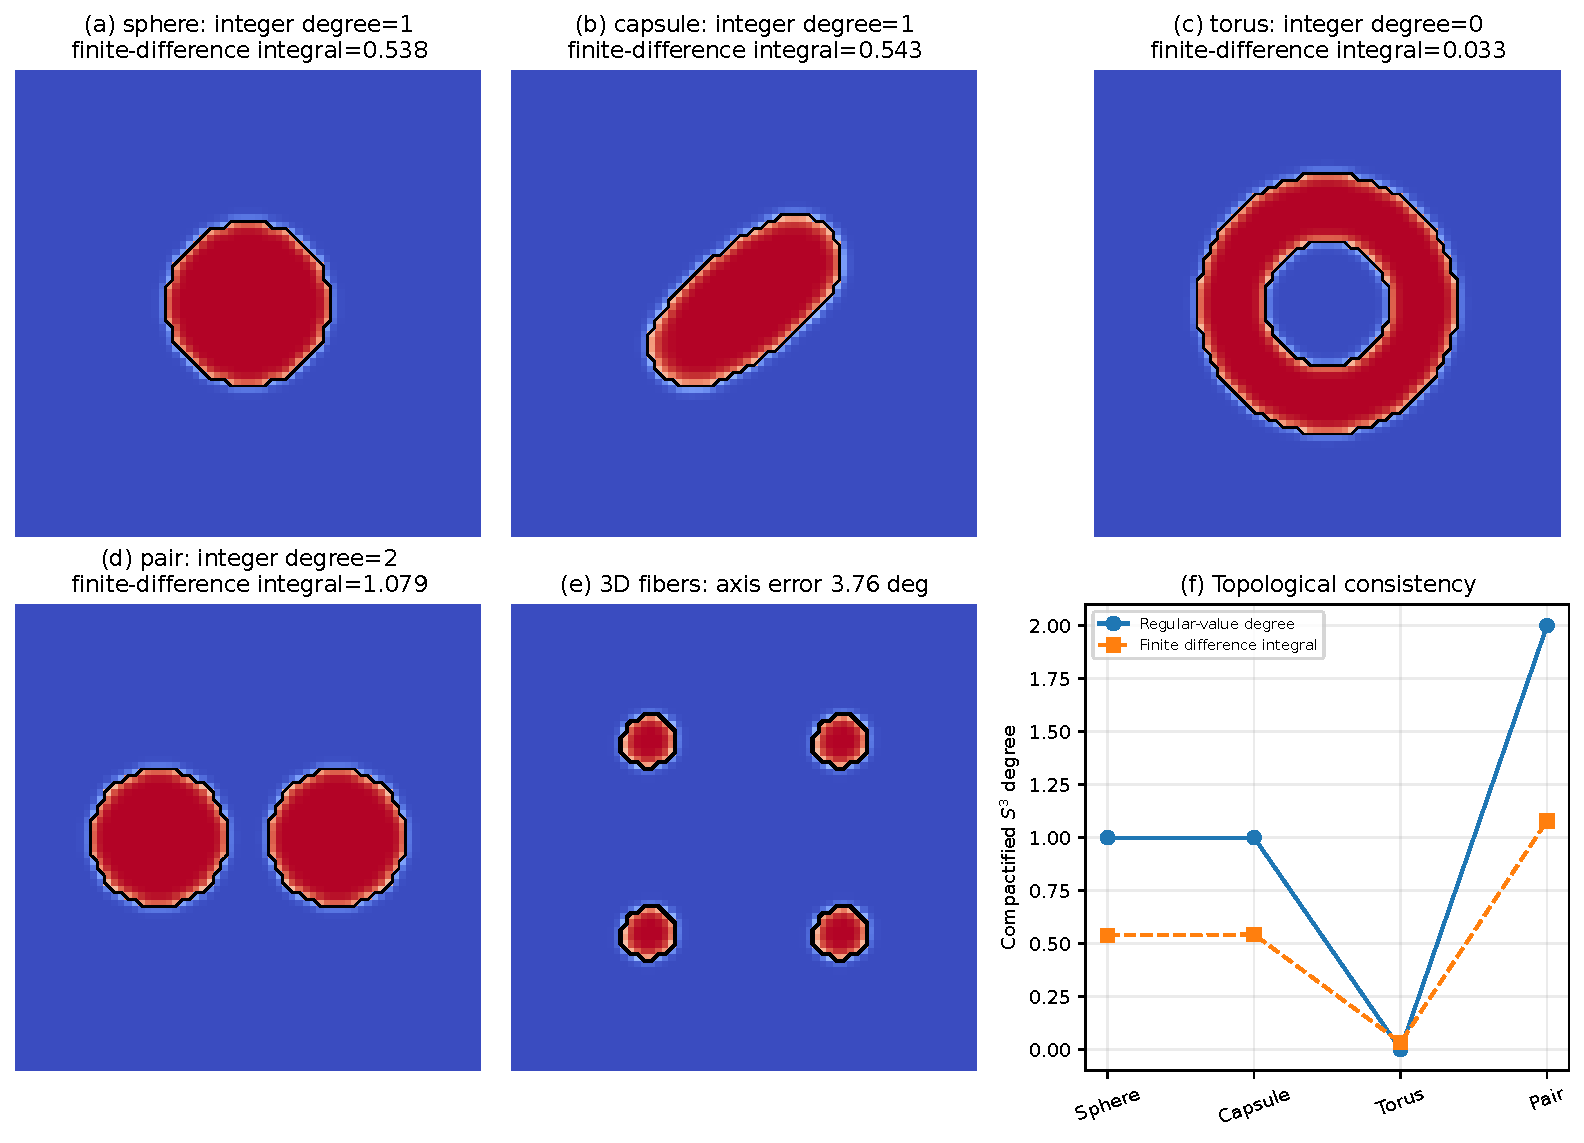
\includegraphics[width=.95\linewidth]{figures/Fig07_3D_generated_Q3.pdf}
\caption{\textbf{Three-dimensional degree calculated from generated four-component spin fields.} (a--d) Central slices of the scalar component $s$ for a sphere, capsule, solid torus, and separated sphere pair. The labels distinguish compactified regular-value integer degree from a direct, coarse-grid determinant integral. (e) Cross section of a synthetic four-fiber volume; the minimum-eigenvalue axis of the transverse normal tensor differs by $3.76^\circ$ from the prescribed fiber direction. (f) Regular-value degrees and finite-difference integral estimates for four shapes. The finite-difference integrals visibly underestimate the degree for these thin grid-scale walls; the integer counts are not rounded versions of those integrals.}
\label{fig:3Dtopo}
\end{figure}

\begin{table}[t]
\centering\caption{\textbf{Selected orientation and topology results.} Direction errors refer to the stated, geometrically defined target. A degree value is neither a universal object count nor a measure of projected director defects.}\label{tab:directiontopology}
\small\begin{tabularx}{\linewidth}{@{}p{.47\linewidth}X@{}}\toprule
Readout and target & Final study result\\\midrule
2D/3D local inward normal cosine & \(0.99378/0.99667\)\\
2D ellipse/stadium Gram-tensor axis error & \(0.205^\circ/0.512^\circ\)\\
3D ellipsoid/capsule Gram-tensor axis error & \(0.332^\circ/0.385^\circ\)\\
Separated pair spatial-covariance axis error & \(0.080^\circ\) (2D), \(0.162^\circ\) (3D)\\
3D \(Q_3\), sphere/capsule/torus/pair & \(1/1/0/2\)\\
New 2D PBGIA generated-field charge (disk/two/ring/mix) & $1/2/0/1$\\\bottomrule
\end{tabularx}
\end{table}

\subsection{Resolution and interpretation}\label{subsec:impl:limits}
The calibrated geometric observables apply to the resolved structures examined here. Objects narrower than the generated interface and objects with indistinguishable pixel masks can produce ambiguous or unstable boundary readouts. These resolution effects were explicitly probed in the frozen benchmark, and supplementary diagnostics are available in its source repository. For degree-based counting, the compactified boundary convention and the selected interpolation must also be specified; our 2D and 3D examples use the same numerical spin-generation rule but separate dimension-appropriate charge evaluators.

\FloatBarrier
\section{Discussion}\label{sec:discussion}
The principal finding is that a binary input can be mapped into a normalized spin field from which several complementary measurements can be extracted. The same field gives a boundary-localized gradient measure for perimeter or surface area, transverse directions for local normals, tensors for spatial orientation, and selected topological descriptors. This common representation connects the magnetic texture and geometric image analysis viewpoints developed in our previous studies \cite{Park2024AMT,Moon2025SR,Park2025iScience}.

The continuum domain-wall model explains why a sharply varying external source produces a smooth boundary texture and why its energy is localized near interfaces. The actual fixed-iteration implementation is an efficient alignment dynamics inspired by this picture rather than an exact minimizer of the displayed continuum Hamiltonian. It provides sub-percent average extent errors for the tested shapes, while direct conventional estimators remain highly competitive when only one geometrical observable is needed. The practical motivation of the spin representation is the possibility of reusing its components for additional measurements.

For orientational information, the relevant quantities are tensorial. A local outer product $\vv\vv^{\mathsf T}$ is unchanged by $\vv\rightarrow-\vv$; its coarse-grained form provides a projective director wherever the principal eigenvalue is distinct. This feature makes directional information available without choosing an artificial sign for a line field. Pooling these tensors across multiple binary thresholds extends the same construction to grayscale textures. The director angle and anisotropy amplitude describe two different aspects of alignment, conveniently shown by segment orientation and length. In synthetic layers and fiber-like images this produces a compact visual summary of their local organization. The CC0 architectural texture additionally provides a controlled demonstration of relative orientation tracking under imposed rotations. The new volumetric fiber array illustrates that a three-dimensional normal tensor can recover a meaningful longitudinal eigenline, complementing the two-dimensional image examples.

The new stadium and 3D examples make the geometric message explicit: a known boundary scale and an independently defined orientation axis can be recovered from the same generated field, while the degree provides a complementary topological summary. The relevant conventions for wall resolution, mixed tensor eigenlines, and compactified degree are described in Methods rather than treating each as a separate limitation of the framework.

The method is therefore most naturally viewed as a reusable physics-based intermediate representation, complementary to contour-based geometry estimators and direct gradient-based orientation methods. Its value is in organizing boundary extent, direction, projective order, and selected topology-related information within a consistent computational field.

\begin{figure}[p]
\centering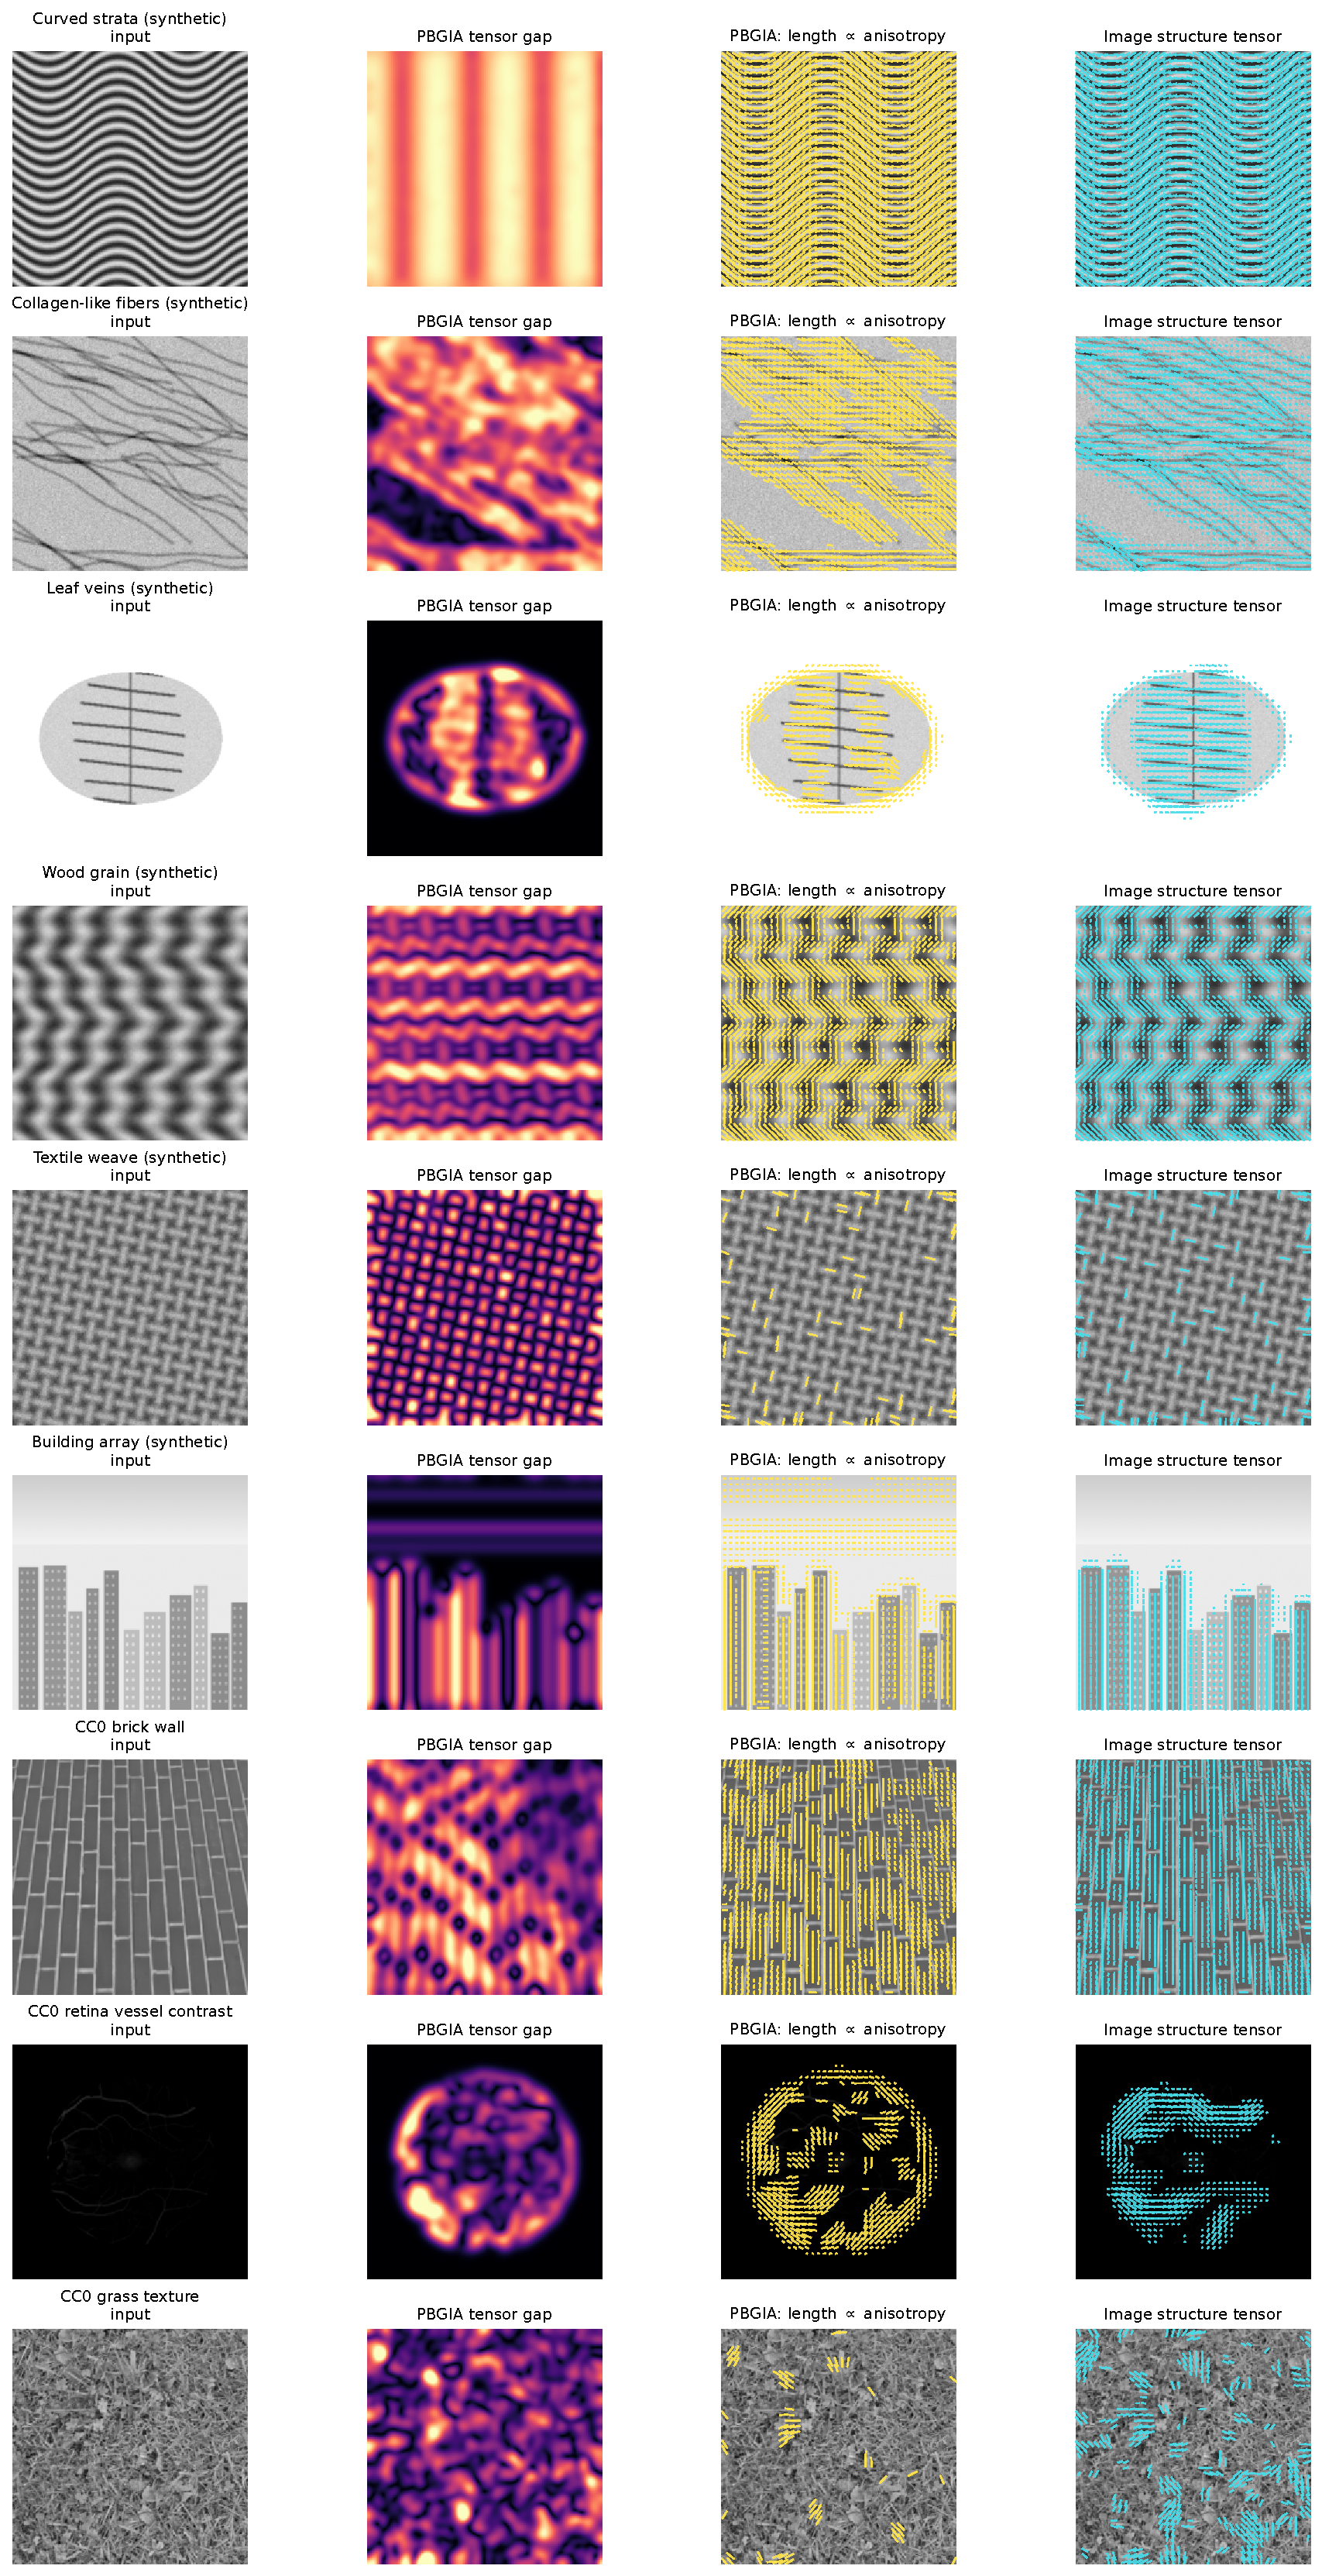
\includegraphics[width=.87\linewidth,height=.83\textheight,keepaspectratio]{figures/FigS_multithreshold_application_gallery.pdf}
\caption{\textbf{Supplementary multi-threshold application gallery.} Input, pooled PBGIA anisotropy $\Delta\lambda$, dense amplitude-scaled PBGIA tangent directors, and conventional intensity structure tensors are shown for nine synthetic or CC0 images. The illustrated cases include synthetic strata, collagen-like fibers, leaf venation, wood grain, woven fabric, and building array, plus CC0 brick wall, retinal image, and grass texture. Line lengths encode within-image tensor anisotropy. Synthetic examples provide illustrative morphology, and the CC0 images provide reproducible image inputs without external orientation annotations.}
\label{fig:suppmulti}
\end{figure}

\section{Methods and reproducibility}\label{sec:methods}
\subsection{Grid initialization and fixed dynamics}
The final reference configuration used the \(N=30\) alignment field of Eqs.~\eqref{eq:updatev}--\eqref{eq:updaten} on square/cubic arrays with positive axial nearest-neighbor sums, \(J=D_{\rm a}=1\), \(h=2\), and \(\varepsilon=10^{-12}\) as the small-field threshold. A raster mask was generated from analytic shapes solely to provide a binary input and continuous ground truth for evaluation. The starting scalar profile was obtained from a binary Euclidean distance transform and a hyperbolic-tangent transformation with initial lattice-width parameter 2.3; the transverse component was initialized along a discrete scalar-gradient direction and the resulting spin was normalized. No analytic ground-truth normal was fed to the generator.

The generation gradient was centered. The frozen observer for \(I_E\) used separately selected 2D/3D derivative stencils with axial offsets \(\pm1,\pm2\) and transverse smoothing; it was not reoptimized during the final study. The TV observable used a distinct fixed fourth-order scalar derivative. Dimensions and physical units were tracked separately for derivative energy and total variation. Shape-specific calibration from the final test was prohibited.

\subsection{Training, validation, and frozen test}
An initial split manifest assigned each prototype and all related poses and noise realizations to one partition. The final study used a new random seed (27111743), separate reserved reference circles/spheres, and a bounded five-value search over the mixture coefficient \(\alpha\). Selection used validation MARE plus a rule excluding excessive degradation within any tested noise stratum; test labels were not used to revise the choice. The final 2D and 3D mixture values were \(0\) and \(0.5\). The source repository provides the complete split protocol, selection freeze, per-shape outputs, and paired bootstrap summaries. The confidence interval for mixture improvement was obtained by resampling prototype units, not individual pose variants.

Noise consisted of independently flipped salt-and-pepper pixels/voxels at 0, 0.2, or 1\%, with a protected outer collar. The ground-truth extent was that of the clean analytic shape. The conventional comparisons include 2D Crofton perimeter and 3D marching-cubes area. A frozen Gaussian smoothing baseline was also studied, but these comparisons were not tuned to establish the optimal conventional pipeline for each data family. Timings were obtained on CPU, with warmup and isolated measurements; hardware and environment details are preserved in the repository.

\subsection{Additional stadium, charge, and 3D-volume calculations}
The new stadium tests were performed on $160^2$ grids using capsule-shaped 2D domains whose two semicircular caps have radius $R$ and center separation $L=2R$. The orientation sweep used $R=17$ and angles $0,15,\ldots,165^\circ$. The principal axis was obtained from spatial covariance weighted by the magnitude of the generated scalar gradient, not from the local normal-tensor eigenvector. The size experiment used nine radii $R=9,11,\ldots,25$ and three rotations $(0,27,54)^\circ$. The raw scalar TV readout was $I_{\rm TV}=\frac12\sum|\nabla s|$ with a basic central-difference gradient; the $R=9$, $0^\circ$ reference alone set its multiplicative coefficient. The fit and MARE were calculated on the remaining eight sizes and 24 poses, independently of the held-out benchmark in Sec.~\ref{subsec:impl:benchmark}.

For the new 2D topology test, every $154^2$ mask was evolved for 30 iterations. The degree was summed from the exact oriented solid angle $\Omega(a,b,c)=2\operatorname{atan2}[a\cdot(b\times c),1+a\cdot b+b\cdot c+c\cdot a]$ of each of two triangles per square, divided by $4\pi$. The accompanying density images use the simpler finite-difference cross-product formula, and the value reported for $Q_2$ is the spherical-triangle integral.

The new $68^3$ synthetic volumes consist of analytically defined solid spheres, a rounded capsule, a solid torus, separated spheres, four non-overlapping rounded fibers, and a Gaussian-field porous structure explored only as a diagnostic. The first five families have explicit analytic areas. They were rasterized before field generation, and the same fixed $N=30$ alignment was applied in three dimensions. A sphere of radius $12$ pixels set one geometric conversion coefficient between a central-gradient integral and interface area; it was not fitted on any of the other shapes. The fiber-axis estimate is the minimum eigenvector of $\sum(1-s^2)\vv\vv^{\mathsf T}$ integrated over the volume. The compactified $S^3$ degree was evaluated using a regular-value intersection count on six Freudenthal tetrahedra per voxel cell, with a fixed three-voxel outer collar; three generic target vectors were used to verify the resulting integer on the reported analytic shapes. Coarse finite-difference determinant integrals were recorded separately to expose quadrature effects and are not substituted for the topological integer. These are generated geometric benchmarks; publicly identified real CT datasets are a natural application target, but no unacquired micro-CT data are presented as measured here.

\subsection{Multithreshold image pilot: preprocessing and fixed comparison}
The image-level pilot is an exploratory extension of the frozen extent benchmark and did not change its geometry or topology results. We used synthetic curves, collagen-like filaments, leaf-like branching veins, weave, wood grain, and schematic building arrays. The real-source images in the study are \texttt{scikit-image} brick texture, retinal fundus photograph, and grass texture, for which the data documentation specifies CC0 provenance \cite{VanderWalt2014}. Images provided in informal discussion under uncertain reuse rights were excluded from all publication figures. Sample arrays, figure-generation scripts, and numerical CSV outputs are included in the companion package.

All grayscale inputs were rescaled to $320\times320$ pixels, intensity-normalized to $[0,1]$, and Gaussian-smoothed with standard deviation $0.8$ pixels. Each image was thresholded at the $15$, $32.5$, $50$, $67.5$, and $85$ intensity percentiles, yielding five \emph{independent} $\mathbb Z_2$ inputs. For color input, the specified reference implementation first converts RGB intensities to luminance using weights $(0.2989,0.5870,0.1140)$; color-channel-specific pooling was not tested. Each threshold mask was initialized from its own Euclidean distance transform, then evolved for $N=30$ normalized updates with $J=D_{\rm a}=1$ and $h=2$. Gaussian-windowed products $v_i v_j$ ($\sigma=8$ pixels) were averaged over thresholds, not the spin components or already extracted eigenvectors. We used threshold count $K=5$ without optimizing the cutoffs against the displayed datasets; the number of thresholds is a numerical illustration rather than an independently selected optimum.

The principal eigenvector of this pooled tensor indicates a local boundary normal; its perpendicular gives the unoriented tangent. We calculated $\Delta\lambda$ and the normalized coherence $c$ from the tensor eigenvalues. Displayed line segments were spaced by six image pixels, with lengths set by Eq.~\eqref{eq:segmentlength}; no arrowheads were plotted. High-confidence selection required $c>0.25$ and $\Delta\lambda/\Delta\lambda_{95}\ge0.07$. We compare the inferred director with a direct intensity structure tensor using the same Gaussian window ($\sigma=8$ pixels) after pre-smoothing ($\sigma=1.2$ pixels). For the sinusoidal strata $y-A\sin(2\pi x/L)=\mathrm{const}$, the analytical tangent field used $A=22$, $L=190$, and a stripe period of 17 pixels; reported local errors were evaluated on the PBGIA confidence-selected subset.

For the relative rotation test, the same $320\times320$ input was rotated at angles of $-15^\circ$, $-10^\circ$, $-5^\circ$, $0^\circ$, $5^\circ$, $10^\circ$, and $15^\circ$ using bilinear interpolation and reflected boundary extension. A global axial average in the central region used $\Delta\lambda$ as weight, and the change relative to the zero-rotation reference was compared to the inserted rotation. For the displayed $+10^\circ$ case, both known rotations were propagated through a binary validity mask, and all four panels were cropped to the common $258\times258$ pixel core without reflected border data. These numbers measure a finite set of interpolation-affected orientation changes; absolute photo leveling or perspective correction was not tested. The gallery of additional image classes and a CSV of all nine pilot metrics are provided as supplements; no unmeasured biological or architectural ground truth is implied.

\subsection{Orientation, projection, degree, and limitations}
The local direction diagnostic compared the generated transverse vector with an analytic inward normal in a narrow band around clean boundaries. The geometry tensor, spatial covariance, and eigenvalue-based orientation targets were evaluated separately, with no arbitrary target axis assigned to isotropic shapes. For the projection study, uniform and \(1-s^2\)-weighted fiber averages were computed along each of the three array axes of six \(40^3\) generated examples. The leading eigenline was displayed only with sufficient trace and a nondegenerate largest eigenvalue under the study's predeclared numerical criteria. The integer \(\Sn^3\) degree was computed after a specified outer-collar compactification and tetrahedral interpolation; multiple target checks and interpolation-regularity diagnostics limited claims to numerically supported endpoints.

The pixel-information experiment constructed pairs of continuous circles and spheres with different physical radii or centers but identical point-sampled raster masks. For each pair, the true geometry was computed analytically and a corresponding two-object minimax error bound was evaluated. A separate high-frequency corrugation example illustrated the failure of unconstrained geometric recovery when subpixel curvature is unbounded. This deliberately pathological example was not treated as representative of naturally smooth objects.

The numerical analyses, figure-generation workflow, and preliminary manuscript drafting used AI-assisted software tools. The scientific interpretations, code verification, authorship, and final responsibility must be reviewed and approved by the named authors before submission. The accompanying final research repository reports a clean sequential reproduction and successful automated tests; our textual draft does not constitute an independent repeat of every experiment.

\section{Conclusion}\label{sec:conclusion}
We have developed and evaluated a route from a spatial binary field to normalized spin textures and their geometric readouts. A simple domain-wall model motivates the boundary-energy relationship, and the discrete algorithm provides quantitative perimeter and surface-area measurements alongside orientation and topology-related observables. New stadium tests link generated-field axes and extent to analytic geometry; numerical $S^2$ and $S^3$ degree tests and synthetic 3D fibers extend the demonstration to counting and volumetric orientation. With multiple intensity thresholds, the same construction yields dense projective director maps in which line direction and length represent local orientation and tensor anisotropy. The results illustrate how a common spin-texture representation can connect geometrical and directional analyses of images across spatial dimensions, while remaining compatible with specialized conventional methods.

\section*{Data and code availability}
The underlying numerical study and reproducibility materials are available in the public repository \url{https://github.com/cywon-commits/Physics-Based-Geometric-Image-Analysis}, at commit \texttt{b2107084d19fcdf54c9350cf3f0e013fed8afa4c}, in \texttt{final\_pbgia\_study/}. The release includes the numerical scripts, frozen selection, test tables, projection diagnostics, pixel-information experiments, and figure data. Large three-dimensional spin checkpoints are not distributed but can be regenerated from the recorded parameters and software environment. New stadium and topology evaluation scripts, synthetic 3D volume generators, orientation-pilot code, the CC0 source-image arrays, and controlled-rotation outputs accompany this manuscript revision and have not yet been committed to the frozen public numerical repository; the authors should archive them with the submission. A permanent archival DOI has not yet been assigned.

\section*{Acknowledgments}
\emph{Funding acknowledgement to be confirmed by the author team.} Previous papers by this group acknowledge support from Korean funding agencies, but the grants applicable to the present work must be verified independently; they are not automatically carried over.

\section*{Author contributions}
\emph{To be completed with the authors' approval, using the CRediT roles if requested by the target journal.}

\section*{Declaration of interests}
\emph{To be completed and confirmed by all authors.}

\section*{Use of generative AI}
AI-assisted tools were used for computational scripting, manuscript drafting, and editorial support as described in Methods. All authors must independently review, correct, and approve the final text, data, and conclusions and follow the selected journal's policy on disclosure of AI-assisted work.

\appendix
\section{Supplementary three-dimensional spin visualization}\label{app:3dvis}
\begin{figure}[h]
\centering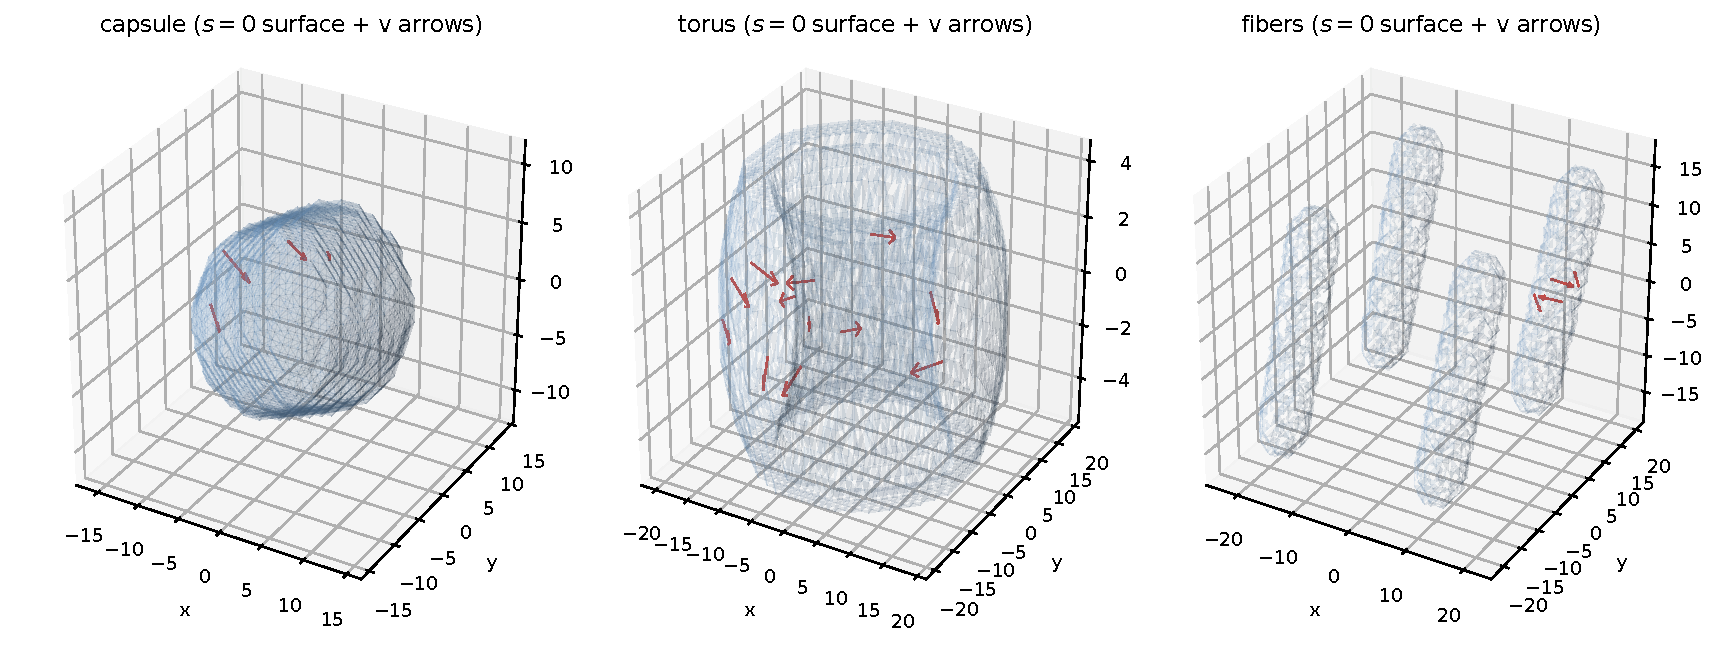
\includegraphics[width=.96\linewidth]{figures/FigS_3D_volume_S3_visualization.pdf}
\caption{\textbf{Illustrative spatial visualization of the numerically generated $S^3$ fields.} Meshes represent the three-dimensional interface of the capsule, solid torus, and four rounded fibers. Arrows show selected samples of the transverse vector $\vv=(v_x,v_y,v_z)$ in a central plane. The fourth spin component $s$ is represented through the interface $s\simeq0$; the numerical state remains a four-component unit vector at every voxel. All examples are newly generated synthetic 3D volumes.}
\label{fig:3Dvis}
\end{figure}


\section{Validity range of the analytic wall approximation}\label{app:wall}
For the step model, Eq.~\eqref{eq:EL} admits a first integral on the positive side of the step,
\begin{equation}
 \frac A2(\theta')^2=h(1-\cos\theta).
\end{equation}
At the wall center the matching condition gives \(\theta(0)=\pi/2\). Integrating \(\dd\theta/(2\sin(\theta/2))=-\dd u/\ell\) yields Eq.~\eqref{eq:wallprofile}. Substituting into the nonchiral energy gives \(\sigma_0=8(1-1/\sqrt2)\sqrt{Ah}\). The DMI term integrates to \(-c\pi D_{\rm c}\) and does not alter this one-dimensional profile for fixed asymptotic spins. The approximation requires a locally planar interface with sufficiently separated walls; in a curved configuration derivatives of \(\bm\nu\) and of the normal-coordinate metric contribute to the energy. Such curvature effects were not eliminated by the train-only calibration.

\section{Distinct meanings of topology in the proposed analysis}\label{app:topology}
A local \(\Sn^d\)-valued spin field, its pointwise \(\RP^d\) projection, a \(\RP^{d-1}\) transverse director, a fiber-averaged tensor eigenline, and the binary object's Euler characteristic are different mathematical objects. In particular, the full pointwise projector \(\nn\nn^{\mathsf T}\) has a globally available lift whenever the spin itself is smooth and nonvanishing, whereas a fiber-averaged tensor can acquire eigenvalue degeneracies and projected eigenline defects without any singularity of the original spin. Furthermore, integer winding in \(\pi_1(\RP^1)\simeq\bbZ\) differs from \(\bbZ_2\) loop classification for \(\RP^m\), \(m\ge2\). The compactified \(\Sn^3\) degree measured in the final 3D study is a separate invariant belonging to \(\pi_3(\Sn^3)\simeq\bbZ\).

\begin{table}[p]
\centering\caption{\textbf{Rotation equivariance of multi-threshold orientation readouts.} Entries are mean absolute errors in the estimated \emph{relative axis shift} under seven imposed rotations from $-15^\circ$ to $+15^\circ$; they are not errors against an absolute orientation ground truth. Each input was processed at five intensity cutoffs. ST: direct grayscale structure tensor.}
\small\begin{tabular}{@{}lrr@{}}\toprule
Texture & PBGIA equivariance error ($^\circ$) & ST equivariance error ($^\circ$)\\\midrule
Synthetic curved strata & 1.80 & 0.22\\
Synthetic collagen-like fibers & 0.43 & 0.22\\
Synthetic leaf-vein analog & 1.15 & 0.45\\
Synthetic wood grain & 1.42 & 0.23\\
Synthetic textile weave & 3.96 & 0.86\\
Synthetic building array & 2.91 & 0.51\\
CC0 brick wall & 2.46 & 0.74\\
CC0 retinal image & 1.22 & 0.72\\
CC0 grass texture & 22.76 & 0.49\\\bottomrule
\end{tabular}
\label{tab:multithresh}
\end{table}

\bibliographystyle{unsrtnat}
\bibliography{refs}
\end{document}
